% CVPR 2025 Paper Template; see https://github.com/cvpr-org/author-kit

\documentclass[10pt,twocolumn,letterpaper]{article}

%%%%%%%%% PAPER TYPE  - PLEASE UPDATE FOR FINAL VERSION
% \usepackage{cvpr}              % To produce the CAMERA-READY version
% \usepackage[review]{cvpr}      % To produce the REVIEW version
\usepackage[pagenumbers]{cvpr} % To force page numbers, e.g. for an arXiv version

% Import additional packages in the preamble file, before hyperref
% %
% --- inline annotations
%
\newcommand{\red}[1]{{\color{red}#1}}
\newcommand{\todo}[1]{{\color{red}#1}}
\newcommand{\TODO}[1]{\textbf{\color{red}[TODO: #1]}}
% --- disable by uncommenting  
% \renewcommand{\TODO}[1]{}
% \renewcommand{\todo}[1]{#1}



% It is strongly recommended to use hyperref, especially for the review version.
% hyperref with option pagebackref eases the reviewers' job.
% Please disable hyperref *only* if you encounter grave issues, 
% e.g. with the file validation for the camera-ready version.
%
% If you comment hyperref and then uncomment it, you should delete *.aux before re-running LaTeX.
% (Or just hit 'q' on the first LaTeX run, let it finish, and you should be clear).
\definecolor{cvprblue}{rgb}{0.21,0.49,0.74}
\usepackage{multirow}
% \usepackage[table,xcdraw]{xcolor}
% \PassOptionsToPackage{table,xcdraw}{xcolor}
\usepackage{arydshln}
\usepackage[pagebackref,breaklinks,colorlinks,allcolors=cvprblue]{hyperref}

\definecolor{Lavender}{RGB}{230, 230, 250}
\definecolor{indigo}{rgb}{0.294, 0.0, 0.51}

%%%%%%%%% PAPER ID  - PLEASE UPDATE
\def\paperID{7721} % *** Enter the Paper ID here
\def\confName{CVPR}
\def\confYear{2025}

\newcommand{\fref}[1]{Figure~\ref{#1}}
\newcommand{\eref}[1]{(\ref{#1})}
\newcommand{\sref}[1]{Section~\ref{#1}}
\newcommand{\tref}[1]{Table~\ref{#1}}
\newcommand{\aref}[1]{Appendix~\ref{#1}}

%%%%%%%%% TITLE - PLEASE UPDATE
\title{AirRoom: Objects Matter in Room Reidentification}

%%%%%%%%% AUTHORS - PLEASE UPDATE
\author{
Runmao Yao \quad
Yi Du \quad
Zhuoqun Chen \quad
Haoze Zheng \quad
Chen Wang \\
Spatial AI \& Robotics (SAIR) Lab, University at Buffalo \\
{\tt\small \{yaorunmao, zhz19231211\}@gmail.com, \{yid, chenw\}@sairlab.org, zhc057@ucsd.edu}
}
% For a paper whose authors are all at the same institution,
% omit the following lines up until the closing ``}''.
% Additional authors and addresses can be added with ``\and'',
% just like the second author.
% To save space, use either the email address or home page, not both
% \and
% Second Author\\
% Institution2\\
% First line of institution2 address\\
% {\tt\small secondauthor@i2.org}
% }

\begin{document}
\maketitle
\begin{abstract}
Fine-tuning provides an effective means to specialize pre-trained models for various downstream tasks. However, fine-tuning often incurs high memory overhead, especially for large transformer-based models, such as LLMs. While existing methods may reduce certain parts of the memory required for fine-tuning, they still require caching all intermediate activations computed in the forward pass to update weights during the backward pass. In~this work, we develop \method, a method to reduce memory usage,  specifically the memory to store intermediate activations, in the fine-tuning of transformer-based models. During the backward pass, \method approximates the gradient computation by backpropagating through just a subset of input tokens. Thus, with \method, only a subset of intermediate activations are cached during the forward pass. Also, \method can be easily combined with existing methods like LoRA, further reducing the memory cost. We evaluate our approach on pre-trained transformer models with up to billions of parameters, considering the performance on multiple downstream tasks such as text classification and question answering in a few-shot learning setup. Overall, \method achieves performance on par with full fine-tuning or representative memory-efficient fine-tuning methods,  while greatly reducing the memory footprint, especially when combined with other methods with complementary memory reduction mechanisms. We hope that our approach will facilitate the fine-tuning of large transformers,  in specializing them for specific domains or co-training them with other neural components from a larger system. Our code is available at \githubURL.
\blfootnote{\textbf{*} Equal contribution}
\end{abstract}
    
\section{Introduction}
\label{sec:intro}

\begin{figure*}[t!]
    \centering
    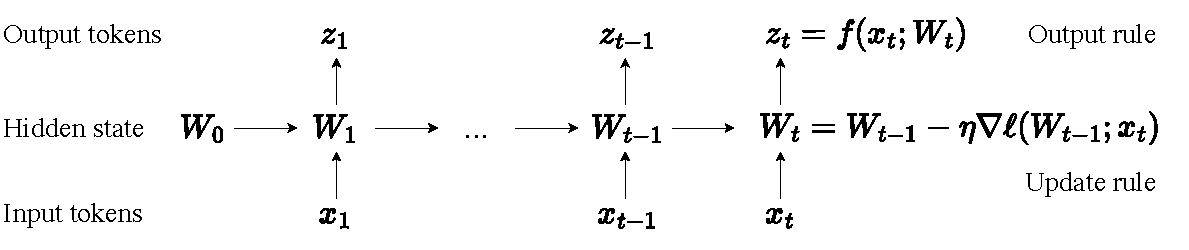
\includegraphics[width=0.8\textwidth]{figs/simple_teaser.pdf}
    \caption{All RNN layers can be expressed as a hidden state that transitions according to an update rule.
    The key idea in \cite{sun2024ttt} is to make the hidden state itself a model $f$ with weights $W$, and the update rule a gradient step on the self-supervised loss $\ell$.
    Therefore, updating the hidden state on a test sequence is equivalent to training the model $f$ at test time. 
    This process, known as Test-Time Training (TTT), is programmed into TTT layers. 
    Figure and caption taken from \cite{sun2024ttt}.
    }
    \label{fig:ttt-layer}
\end{figure*}

Despite the remarkable progress in visual and physical realism, state-of-the-art video Transformers are still generating mostly short clips of single scenes without complex stories.
At the time of writing (March 2025), the maximum length of public APIs for video generation is 20 seconds for Sora (OpenAI), 16 seconds for MovieGen (Meta), 10 for Ray~2 (Luma), and 8 for Veo~2 (Google).
None of these APIs can autonomously generate complex multi-scene stories.

A fundamental challenge behind these technical limitations is long context, because the cost of self-attention layers in Transformers increases quadratically with context length.
This challenge is especially acute for video generation with dynamic motion, whose context cannot be easily compressed by a tokenizer.
Using a standard tokenizer, each of our one-minute videos requires over 300k tokens in context. 
With self-attention, generating a one-minute video would have taken $11\times$ longer than generating 20 videos of 3 seconds each, and training would have taken $12\times$ longer.

To address this challenge, recent work on video generation has investigated RNN layers as an efficient alternative to self-attention, because their cost increases linearly with context length~\cite{wang2024lingenhighresolutionminutelengthtexttovideo}.
Modern RNN layers, especially variants of linear attention~\cite{schmidhuberlinearattn, katharopoulos2020lineartransformers} such as Mamba~\cite{gu2024mamba, dao2024mamba2} and DeltaNet~\cite{schlag2021deltanet, yang2025gateddeltanetworksimproving}, have shown impressive results for natural language tasks.
However, we have yet to see long videos with complex stories or dynamic motion generated by RNNs.
Videos (\href{https://lineargen.github.io/}{link}) in \cite{wang2024lingenhighresolutionminutelengthtexttovideo} are high resolution and one-minute long, but contain only single scenes and slow motion, let alone complex stories.

We believe that these RNN layers generate less complex videos because their hidden states are less expressive.
RNN layers can only store past tokens into a hidden state of fixed size, which is only a matrix for linear attention variants such as Mamba and DeltaNet.
It is inherently challenging to compress hundreds of thousands of vectors into a matrix with only thousands in rank.
As a consequence, these RNN layers struggle to remember the deep relationships between distant tokens.

We experiment with an alternative class of RNN layers whose hidden states themselves can be neural networks. Specifically, we use two-layer MLPs with 2$\times$ more hidden cells and richer nonlinearities than the linear (matrix) hidden states in linear attention variants.
Since the neural network hidden states are updated by training even on test sequences, these new layers are called Test-Time Training (TTT) layers~\cite{sun2024ttt}.

We start from a pre-trained Diffusion Transformer (CogVideo-X 5B \cite{hong2023cogvideo}) that could only generate 3-second short clips at 16 fps (or 6 seconds at 8 fps).
Then, we add TTT layers initialized from scratch and fine-tune this model to generate one-minute videos from text storyboards. 
We limit the self-attention layers to 3-second segments so their cost stays manageable.
With only preliminary systems optimization, our training run takes the equivalent of 50 hours on 256 H100s.

We curate a text-to-video dataset based on $\approx$ 7 hours of \textit{Tom and Jerry} cartoons with human-annotated storyboards.
We intentionally limit our scope to this specific domain for fast research iteration.
As a proof-of-concept, our dataset emphasizes complex, multi-scene, and long-range stories with dynamic motion, where progress is still needed; it has less emphasis on visual and physical realism, where remarkable progress has already been made.
We believe that improvements in long-context capabilities for this specific domain will transfer to general-purpose video generation.

Compared to strong baselines such as Mamba 2~\cite{dao2024mamba2}, Gated DeltaNet~\cite{yang2025gateddeltanetworksimproving}, and sliding-window attention layers, TTT layers generate much more coherent videos that tell complex stories with dynamic motion, leading by 34 Elo points in a human evaluation of 100 videos per method.
For context, GPT-4o scores 29 Elo points over GPT-4 Turbo in LMSys Chatbot Arena~\cite{chiang2024chatbot}.

Sample videos, code and annotations are available at:
\url{https://test-time-training.github.io/video-dit}
\section{Related Work}
\label{sec:related_work}

In this section, we review areas mostly related to our work, \ie, image retrieval and visual place recognition.

\subsection{Image Retrieval}

Image retrieval is a fundamental and well-established task in computer vision that involves searching for images similar to a given query within a large database.
The process of image retrieval typically consists of two stages: global retrieval and re-ranking. In the first stage, a global descriptor that aggregates local features is used to retrieve $k$ candidates from a large database. This is followed by spatial verification through local feature matching to re-rank these $k$ candidates. Early research relied on handcrafted features \cite{Lowe2004DistinctiveIF, BAY2008346}, while current methods utilize deep networks to learn informative representations \cite{cao2020unifyingdeeplocalglobal, radenović2018finetuningcnnimageretrieval}.

Most image retrieval methods focus on selecting diverse relevant images to help users discover options that align with their interests or needs in real-world applications \cite{Wan2014DeepLF}. Although these methods are effective in retrieving similar images, they often lack the emphasis on distinguishing between categories or achieving precise ReID \cite{10.1145/1348246.1348248}.
In \mbox{contrast}, our approach prioritizes achieving accurate ReID. Following a ``global retrieval and re-ranking" pipeline, we first use global context features to identify the top five room candidates. Our object-aware mechanism then refines the search in a coarse-to-fine manner, progressively distinguishing among candidates until the most similar room is \mbox{identified}, yielding accurate results.

\begin{figure*}[ht]
    \centering
    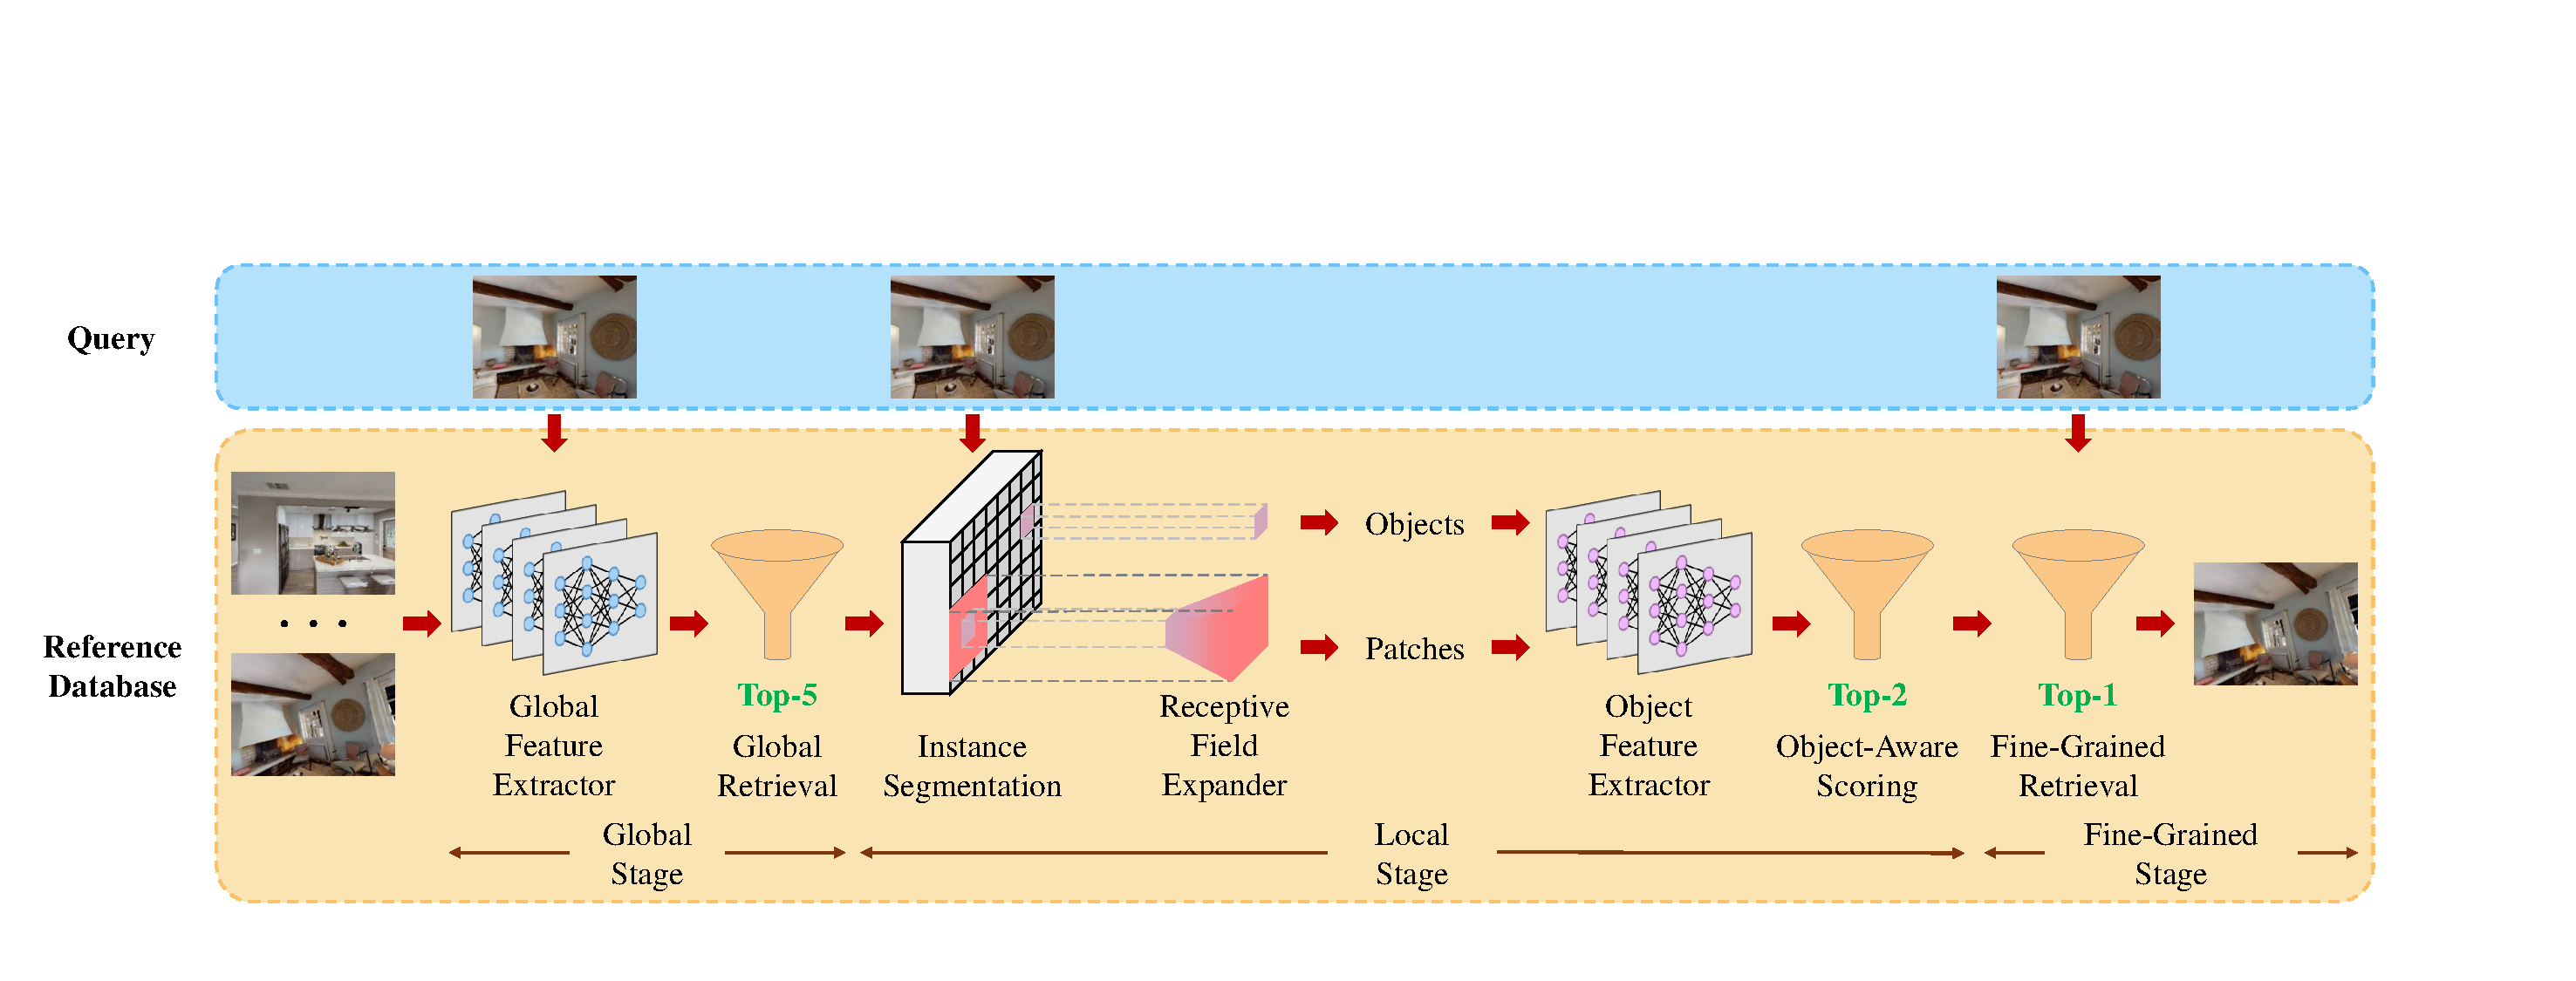
\includegraphics[width=\textwidth]{pipeline_font.pdf}
    \vspace{-16pt}
    \caption{\textbf{The AirRoom coarse-to-fine pipeline}. The pipeline begins with the Global Feature Extractor, which captures global context features to retrieve the top-5 reference images. Instance segmentation then generates object masks, followed by the Receptive Field Expander, which extracts object patches. The Object Feature Extractor processes both object and patch features. The Object-Aware Scoring module narrows the selection to the top-2 candidates, and Fine-Grained Retrieval identifies the most suitable reference image.}
    \vspace{-15pt}
    \label{fig:pipeline}
\end{figure*}

\subsection{Visual Place Recognition}

Visual place recognition (VPR) is often framed as a special image retrieval problem, aiming to match a view of a location with an image of the same place taken under different conditions.
Previous methods fall into two categories: those that directly use global descriptors and those that aggregate local features into a global descriptor. Earlier approaches that relied on global descriptors primarily used CNN-based backbones, such as ResNet \cite{he2015deepresiduallearningimage}, to generate these descriptors. More recent methods, however, leverage foundation models like DINOv2 \cite{oquab2024dinov2learningrobustvisual} for enhanced feature representation. In the aggregation category, early techniques employed handcrafted features like SIFT \cite{Lowe2004DistinctiveIF}, SURF \cite{10.1007/11744023_32}, and ORB \cite{6126544}. Later advancements, including the NetVLAD series \cite{arandjelović2016netvladcnnarchitectureweakly, hausler2021patchnetvladmultiscalefusionlocallyglobal} and AnyLoc \cite{keetha2023anylocuniversalvisualplace}, adopted learning-based models to extract feature maps and combine local features into comprehensive global descriptors.

However, the high performance of most VPR approaches is largely attributed to large-scale training on VPR-specific datasets \cite{keetha2023anylocuniversalvisualplace}. Collecting extensive data for outdoor scenes is relatively straightforward due to natural variations in daylight, weather, and seasons. However, such data collection is more challenging in indoor rooms, making large-scale training on indoor datasets difficult and potentially limiting their effectiveness.
Our approach effectively tackles this challenge by focusing on object-oriented feature representations, allowing us to leverage mature, pre-trained models for object feature learning. This design enables AirRoom to deliver robust performance without requiring any additional training or fine-tuning on specific datasets.
% Our approach addresses this challenge by centering on objects within indoor spaces, leveraging object-related feature representations. Additionally, AirRoom benefits from mature, pre-trained models for object-centric feature learning. This design enables our approach to deliver robust performance without the need for additional training or fine-tuning on specific datasets.
\section{Proposed Approach}
\label{sec:proposed_approach}

We propose a simple yet highly effective pipeline, AirRoom, for room reidentification that leverages multi-level object-oriented information, as shown in \fref{fig:pipeline}. We will now systematically introduce each module of the pipeline, following the sequence of stages in which they are executed.

\subsection{Global Stage}

In this stage, we utilize the Global Feature Extractor to capture global context features, which are derived from the collective presence of objects within the room. These features are then used for Global Retrieval, coarsely selecting semantically similar candidate rooms from the database.

\subsubsection{Global Feature Extractor}
\label{sec:section3.1.1}

Indoor rooms exhibit fewer variations compared to outdoor environments. They lack diverse topographies, such as aerial, subterranean, or underwater features, and do not experience temporal changes like day-night or seasonal variations. Consequently, collecting large datasets for each indoor room is challenging, complicating large-scale training as seen in many VPR methods \cite{arandjelović2016netvladcnnarchitectureweakly, hausler2021patchnetvladmultiscalefusionlocallyglobal, alibey2023mixvprfeaturemixingvisual}. 

However, indoor rooms are inherently rich in objects, each contributing to the room’s overall semantic context. By leveraging this global context information, we can refine the reference search to specifically focus on rooms with similar semantic features to those in the query image. For this purpose, we prefer backbones pretrained on large image datasets, as they provide strong generalizability and effectively capture informative global context features \cite{kornblith2019betterimagenetmodelstransfer}. Our model selections, therefore, include pretrained CNN-based models such as ResNet \cite{he2015deepresiduallearningimage} and transformer-based self-supervised models like DINOv2 \cite{oquab2024dinov2learningrobustvisual}.

\subsubsection{Global Retrieval}

Using the Global Feature Extractor, we extract global context features for \(M\) query and \(N\) reference images. Let \(\mathbf{Q} \in \mathbb{R}^{M \times D_g}\) and \(\mathbf{R} \in \mathbb{R}^{N \times D_g}\) denote the query and reference features, respectively, where \(D_g\) is the feature dimension. The cosine similarity matrix \(\mathbf{S}\) is then computed as:
% Using the Global Feature Extractor, we first extract global context features for \(M\) query and \(N\) reference images. Given \(M\) query features \(\mathbf{Q} \in \mathbb{R}^{M \times D_g}\) and \(N\) reference features \(\mathbf{R} \in \mathbb{R}^{N \times D_g}\), where \(D_g\) denotes the global context feature dimension, we have a cosine similarity matrix \(\mathbf{S}\):
\begin{equation}
    \mathbf{S}_{ij} = \frac{\mathbf{Q}_i \cdot \mathbf{R}_j}{\|\mathbf{Q}_i\| \|\mathbf{R}_j\|}.
    \label{eq:global feature cosine similarity}
\end{equation}
For each query, we select the top-5 most similar reference candidates using the following formula:
\begin{equation}
    \text{Top}_5(\mathbf{S}_{i, :}) = \text{argsort}(-\mathbf{S}_{i, :})[:5],
    \label{eq:global retrieval}
\end{equation}
where \(\mathbf{S}_{i, :}\) represents the cosine similarity for the \(i\)-th query.

\subsection{Local Stage}

Global context features provide valuable semantic information that helps narrow down the candidate list. However, when faced with many semantically similar rooms, relying solely on global context is insufficient, and local features become increasingly essential. In this stage, we adopt a local perspective by first applying instance segmentation and the Receptive Field Expander to identify objects and patches. We then use the Object Feature Extractor to extract features from both objects and patches, followed by Object-Aware Scoring to further refine the candidate list.

\subsubsection{Instance Segmentation}

For each query image and its corresponding five candidates, we employ instance segmentation methods, such as Mask R-CNN \cite{he2018maskrcnn} and Semantic-SAM \cite{li2023semanticsamsegmentrecognizegranularity}, to identify and delineate individual objects. This process generates each object's mask and bounding box. Next, we calculate the center point \(c\) of each object using its bounding box, as shown below:

\begin{equation}
    c = (\frac{x+W}{2}, \frac{y+H}{2}).
    \label{eq:center point}
\end{equation}
In this equation, \(x\) and \(y\) represent the pixel coordinates of the top-left corner of the bounding box, while \(W\) and \(H\) denote the width and height of the bounding box, respectively.

\subsubsection{Receptive Field Expander}

Single object information alone is not sufficiently discriminative. For example, although different desks may have distinct appearances, they can be found in both dining halls and offices. However, when an object is connected with its neighboring items—such as a desk alongside a computer, keyboard, or notebook—it suggests that the room is more likely to be an office rather than a dining hall. This insight motivates us to expand the receptive field from a single object to a patch containing multiple objects.

Given the center points of all objects in an image, we employ Delaunay triangulation \cite{10.5555/1370949} to generate a triangulated graph of object relationships. Specifically, Delaunay triangulation is applied to the set of object centers, ensuring that no object centers are inside the circumcircle of any triangle. This method maximizes the minimum angle of the triangles, preventing narrow, elongated triangles and ensuring more uniform object adjacency. By analyzing the adjacency relationships among the resulting triangles, we can construct the object adjacency matrix, which encodes the spatial and relational proximity of objects within the room.

\vspace{-10pt}
\begin{figure}[ht]
    \centering
    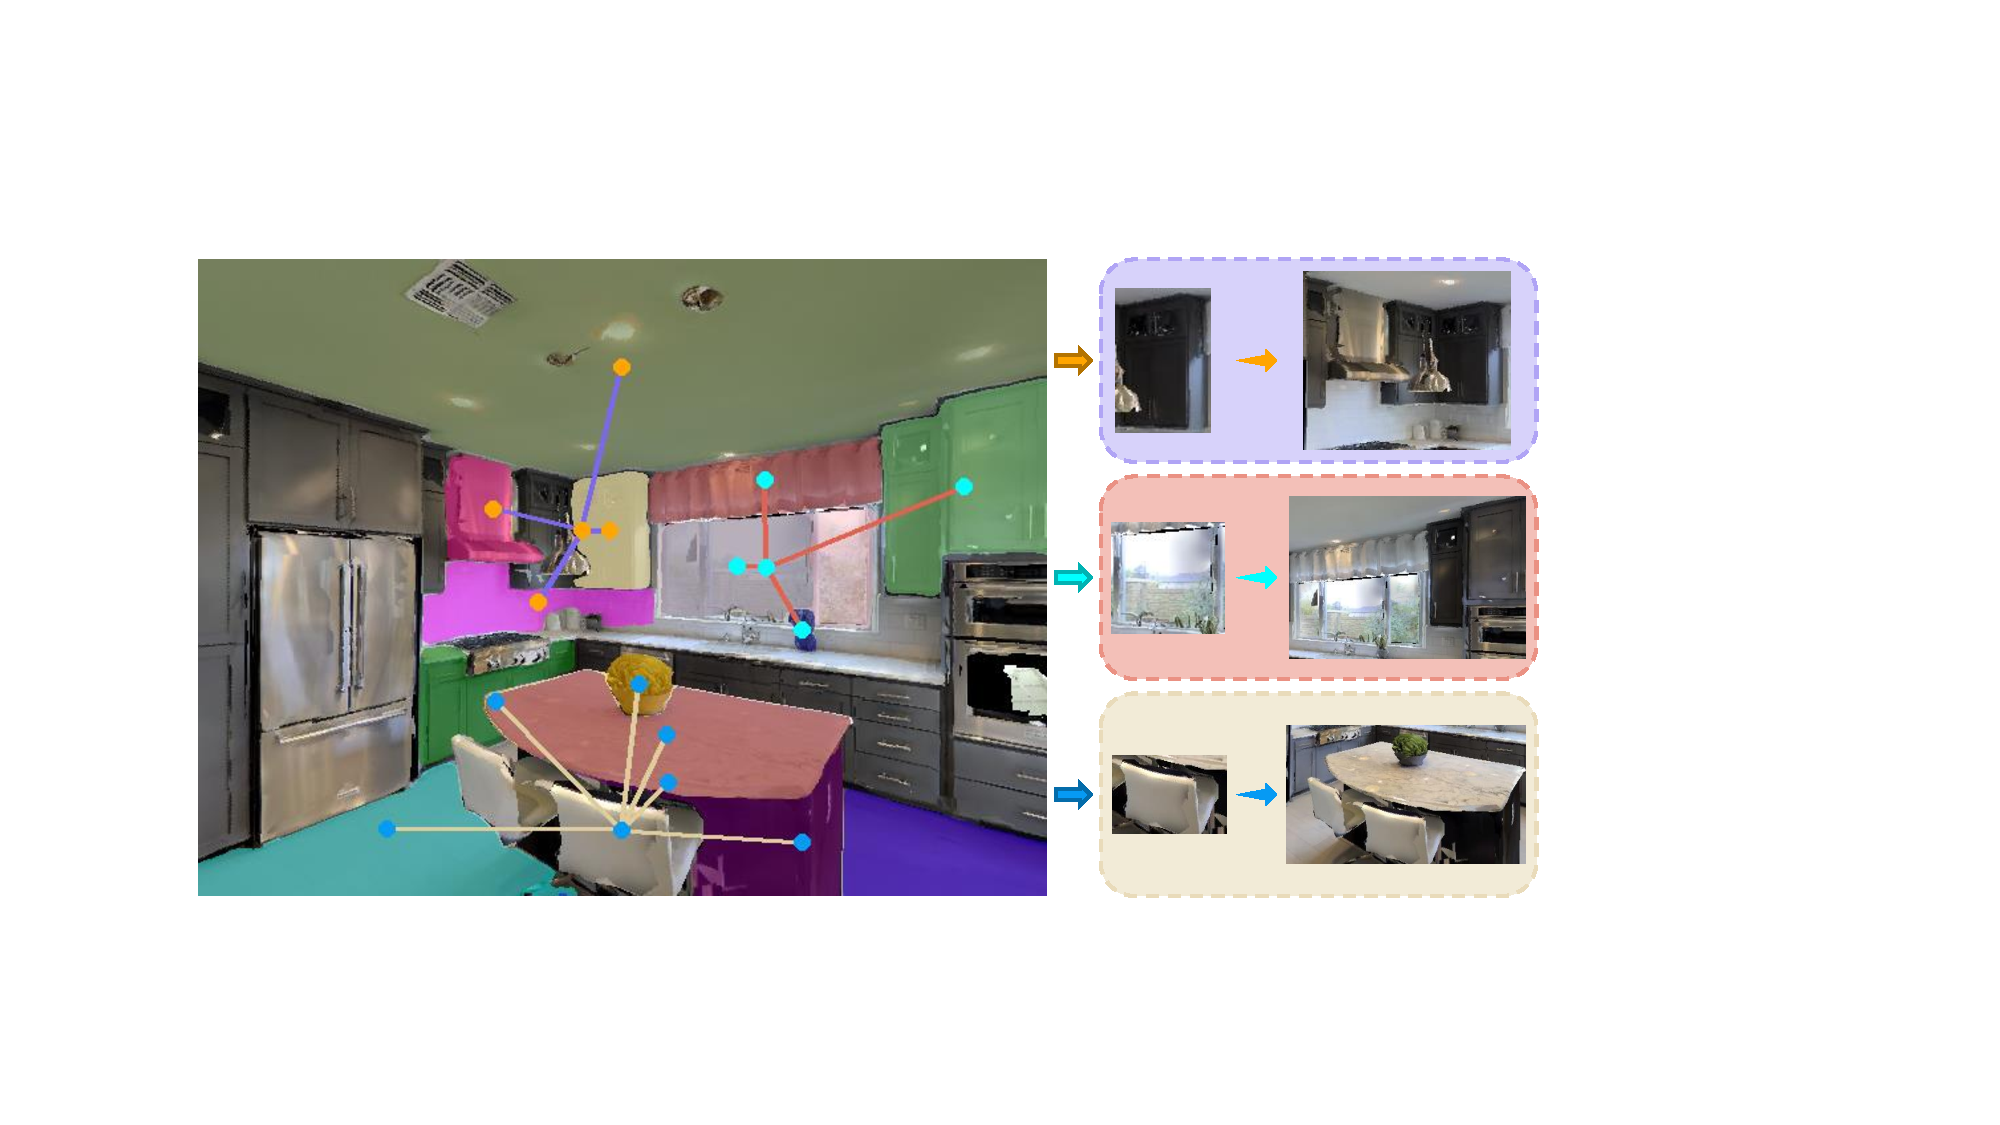
\includegraphics[width=\columnwidth]{expander.pdf}
    \vspace{-20pt}
    \caption{The Receptive Field Expander broadens the receptive field from individual objects to patches rich in contextual information. Leveraging the object adjacency matrix and each object's bounding box, it expands single objects such as a cupboard, window pane, and chair into object patches like a modular kitchen, multi-pane window, and dining set, respectively.}
    \vspace{-5pt}
    \label{fig:expander_image}
\end{figure}

% Given the center points of all objects in an image, we use Delaunay triangulation to create the object adjacency matrix. This mathematical technique takes a set of discrete points and generates triangles that maximize the minimum angle of each triangle, thus avoiding narrow shapes. A key property of Delaunay triangulation is that no discrete point lies within the circumcircle of any triangle formed in the process. By analyzing the adjacency relationships of the triangles created through Delaunay triangulation, we can construct the object adjacency matrix.

Given the object adjacency matrix and bounding boxes in an image, for each object, we consider the bounding boxes of its neighboring objects and enlarge the current object's bounding box to encompass all adjacent objects. This expansion increases the receptive field, enabling us to capture richer contextual information, as illustrated in \fref{fig:expander_image}. We then apply Non-Maximum Suppression (NMS) to select the highest confidence bounding boxes, removing overlapping ones based on their Intersection over Union (IoU) scores. This results in a set of clean, informative object patches.

\begin{figure*}[t]
    \centering
    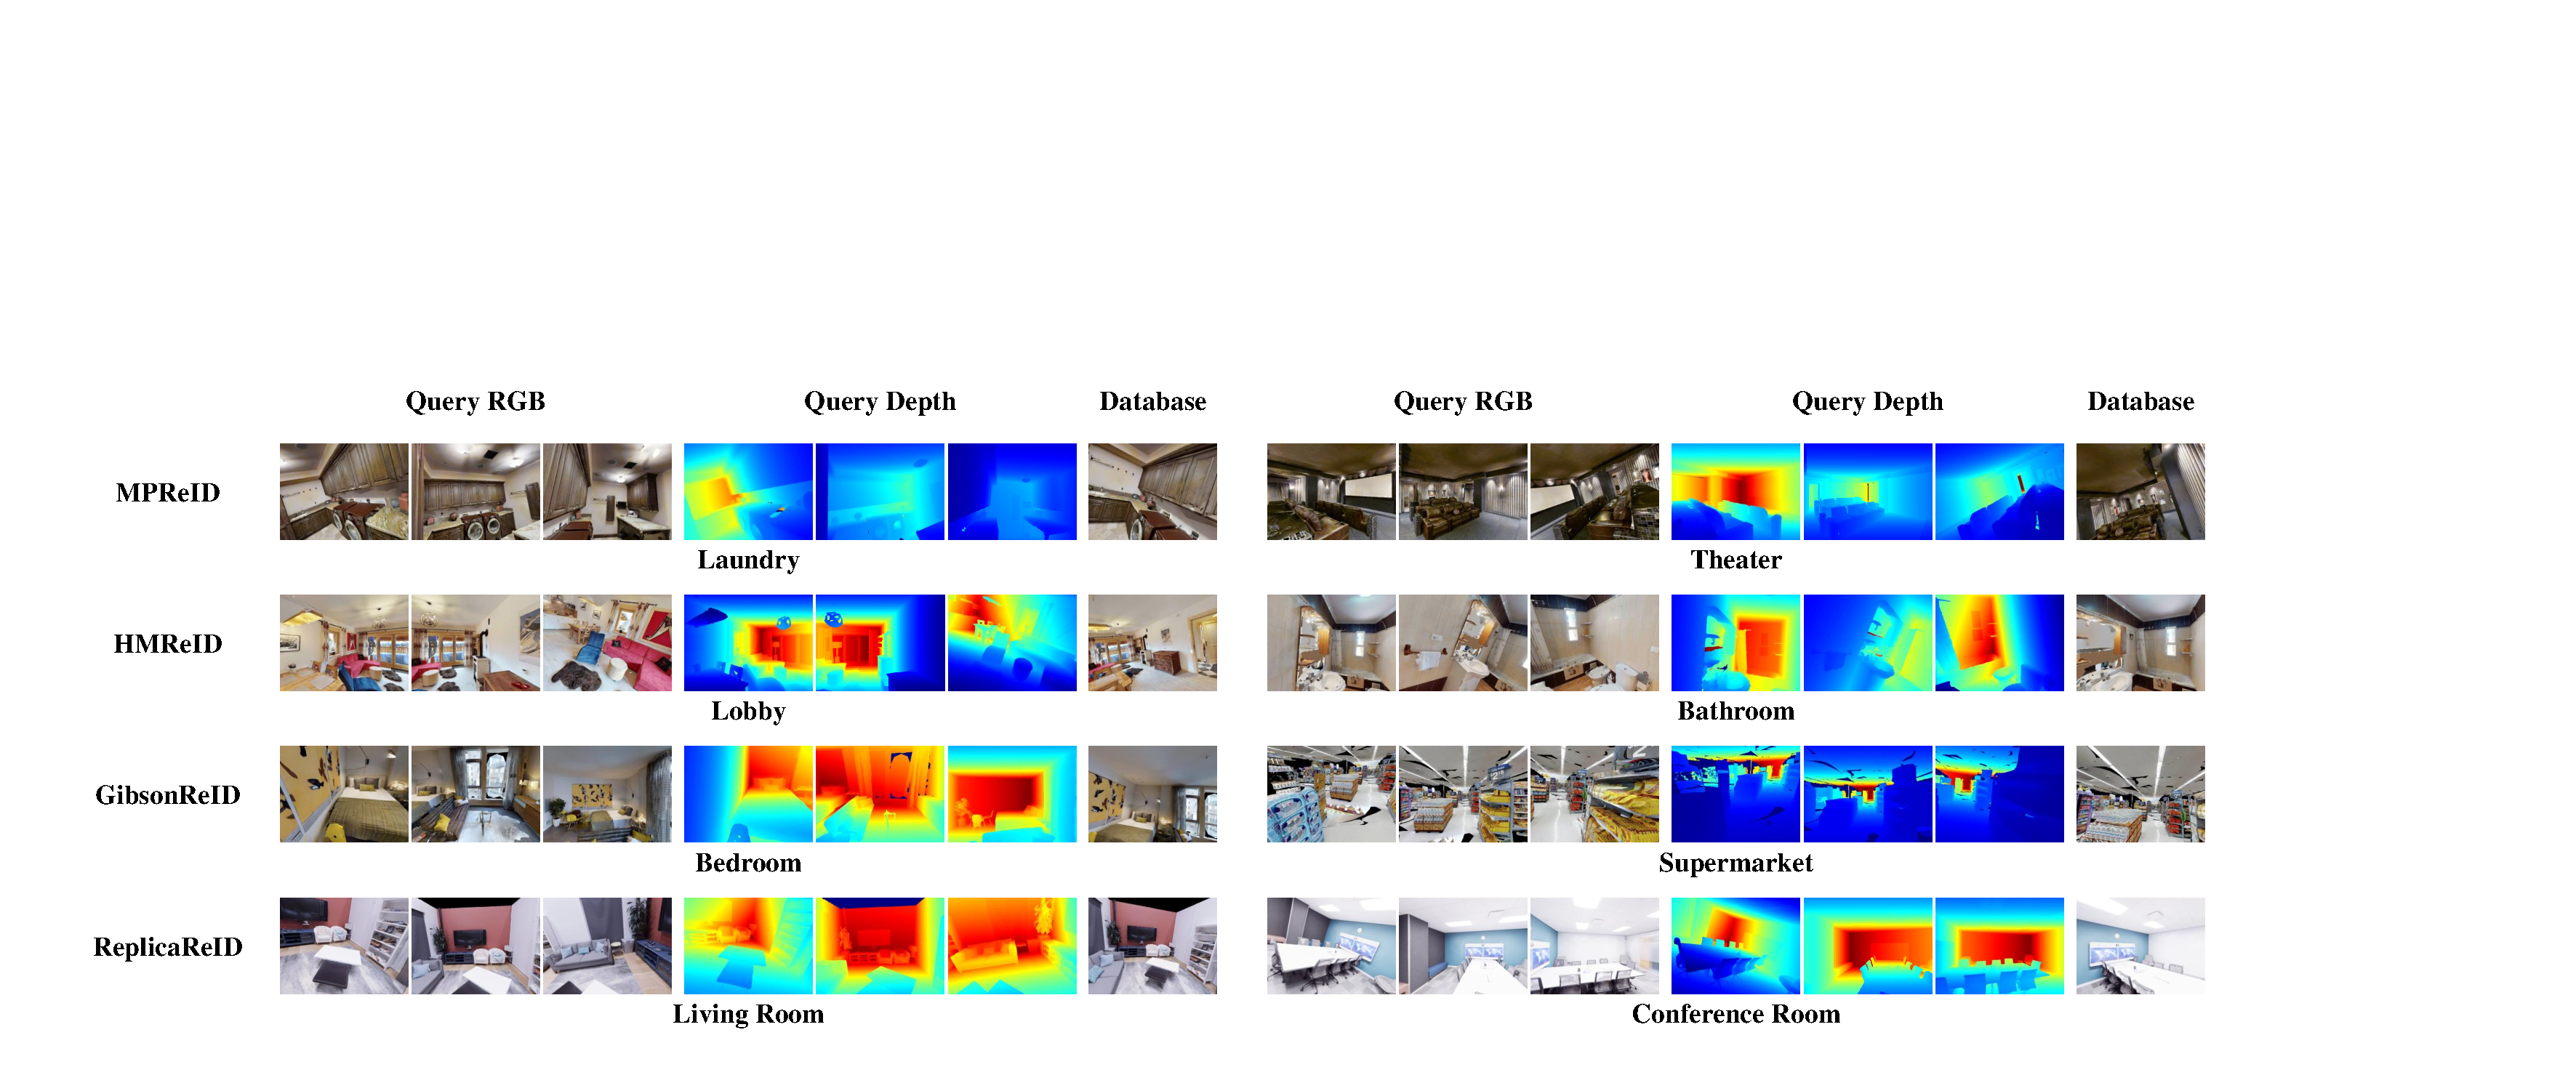
\includegraphics[width=\textwidth]{dataset_font.pdf}
    \vspace{-20pt}
    \caption{Illustration of four newly constructed room reidentification datasets: MPReID, HMReID, GibsonReID, and ReplicaReID. Each room provides only one reference image in the database, while query images for each room capture varied viewpoints.}
    \vspace{-10pt}
    \label{fig:dataset_image}
\end{figure*}

\subsubsection{Object-Aware Refinement}
\label{subsec:refinement}

The Object-Aware Refinement module is composed of three key submodules: Object Feature Extractor, Mutual Nearest Neighbors, and Object-Aware Scoring.

\vspace{-6pt}
\paragraph{Object Feature Extractor}

To effectively leverage object patches and object segmentation information, we prioritize global features over local feature aggregation. The latter approach may fail to capture object characteristics effectively and can significantly increase computational complexity and storage demands \cite{zheng2018sift}. As discussed in Section~\ref{sec:section3.1.1}, we continue to rely on models pre-trained on large image datasets. Using the Object Feature Extractor, we obtain features for both query and reference patches and objects. Let \(Q_p=\{\mathbf{p_i^q}\}_{i=1}^{n_{qp}}\) and \(Q_o=\{\mathbf{o_i^q}\}_{i=1}^{n_{qo}}\) represent the query patch and object feature sets, respectively. For each reference image among the query’s five \mbox{candidates}, we define the reference patch and object feature sets as \(R_p=\{\mathbf{p_i^r}\}_{i=1}^{n_{rp}}\) and \(R_o=\{\mathbf{o_i^r}\}_{i=1}^{n_{ro}}\).

\vspace{-6pt}
\paragraph{Mutual Nearest Neighbors} Given a set of query features \(\{\mathbf{f_i^q}\}_{i=1}^{n_q}\) and reference features \(\{\mathbf{f_i^r}\}_{i=1}^{n_r}\), we obtain feature pairs by identifying mutual nearest neighbor matches through exhaustive comparison of the two sets. Let \(P\) denote the set of cosine similarity scores for these mutual nearest neighbor matches, then we have
\begin{equation}
    P = \{\cos(\mathbf{f_i^q}, \mathbf{f_j^r}) \mid i = \text{NN}_r(\mathbf{f_j^r}), \; j = \text{NN}_q(\mathbf{f_i^q})\}
    \label{eq:mutual nearest neighbors}
\end{equation}
where
\begin{equation}
    \text{NN}_q(\mathbf{f_i^q}) = \arg\max_{j} \left( \frac{\mathbf{f_i^q} \cdot \mathbf{f_j^r}}{\|\mathbf{f_i^q}\| \|\mathbf{f_j^r}\|} \right),
\end{equation}
\begin{equation}
    \text{NN}_r(\mathbf{f_i^r}) = \arg\max_{j} \left( \frac{\mathbf{f_i^r} \cdot \mathbf{f_j^q}}{\|\mathbf{f_i^r}\| \|\mathbf{f_j^q}\|} \right),
\end{equation}
\begin{equation}
    \cos(\mathbf{f_i^q}, \mathbf{f_j^r}) = \frac{\mathbf{f_i^q} \cdot \mathbf{f_j^r}}{\|\mathbf{f_i^q}\| \|\mathbf{f_j^r}\|}.
\end{equation}
% By utilizing mutual nearest neighbors, we can improve retrieval accuracy while narrowing the search space and enhancing retrieval efficiency \cite{zhong2017reranking}.
By utilizing mutual nearest neighbors, we can significantly improve retrieval accuracy, simultaneously narrowing the search space and enhancing overall retrieval efficiency \cite{zhong2017reranking}.

\vspace{-6pt}
\paragraph{Object-Aware Scoring} The object-aware score \(s\) is the sum of the global score \(s_{\text{global}}\) (calculated in Equation~\ref{eq:global feature cosine similarity}), the patch score \(s_{\text{patch}}\), and the object score \(s_{\text{object}}\):
\begin{equation}
    s = s_{\text{global}} + s_{\text{patch}}(Q_p, R_p) + s_{\text{object}}(Q_o, R_o).
    \label{eq:object-aware scoring}
\end{equation}
Here, \(s_{\text{patch}}\) and \(s_{\text{object}}\) can either be \(s_{\text{mean}}\) or \(s_{\max}\), where
\begin{subequations}
\begin{align}
    s_{\text{mean}}(Q_t, R_t) &= \frac{1}{|P(Q_t, R_t)|} \sum_{x \in P(Q_t, R_t)} x,
    \label{eq:mean}\\
    s_{\max}(Q_t, R_t) &= \max_{x \in P(Q_t, R_t)} x.
    \label{eq:max}
\end{align}
\end{subequations}
In these equations, \(P\) denotes the set of cosine similarity scores for mutual nearest neighbor matches, with \(Q_t\) representing either \(Q_p\) or \(Q_o\), and \(R_t\) representing either \(R_p\) or \(R_o\). The global score \(s_{\text{global}}\) serves as a prior, indicating that the initial five candidates vary in relevance. Thus, we retain this term to account for their differing levels of relevance.

\vspace{-8pt}
\paragraph{Object-Aware Refinement} For each query, we select the top-2 most similar reference candidates from the initial five using the Object-Aware Scoring:
\begin{equation}
    \text{Top}_2(\mathbf{s}_{i}) = \text{argsort}(-\mathbf{s}_{i})[:2],
\end{equation}
where \(\mathbf{s}_{i}\) is the object-aware scores for the \(i\)-th query.

\subsection{Fine-Grained Stage}

Patch and object features provide valuable information for understanding the room layout; however, they may be insufficient when distinguishing highly visually similar rooms, particularly in the presence of viewpoint variations and occlusions. Keypoints on objects, by contrast, exhibit strong robustness to texture and appearance variations, enabling them to effectively handle partial occlusions and reject outliers \cite{1498756}. This allows keypoints to offer a more refined approach, capturing finer details for more accurate room identification. In this stage, we use Fine-Grained Retrieval to select the final top-1 result.

\subsubsection{Fine-Grained Retrieval}

Deep matchers, such as SuperGlue \cite{sarlin2020supergluelearningfeaturematching}, perform well in visual localization tasks under challenging conditions, both indoors and outdoors. However, they tend to face efficiency issues. In contrast, LightGlue \cite{lindenberger2023lightgluelocalfeaturematching} offers high efficiency without compromising matching accuracy, making it an ideal choice for our Fine-Grained Retrieval.

For each query image and its two candidate reference images, we match the query to each candidate and record the number of matching keypoint pairs. A higher number of matches typically indicates greater overlap and consistency between the features of the two images, suggesting a higher degree of similarity in their content \cite{Lowe2004DistinctiveIF}. The candidate with more matches is selected as the final result.

\vspace{-3pt}
\section{Experimental Results}
\label{sec:experimental_results}

\begin{table*}[t]
\centering
\resizebox{\textwidth}{!}{%
\begin{tabular}{l|cccc|cccc|cccc|cccc}
\toprule
\multirow{2}{*}{\textbf{Methods}} & \multicolumn{4}{c|}{\textbf{MPReID}} & \multicolumn{4}{c|}{\textbf{HMReID}} & \multicolumn{4}{c|}{\textbf{GibsonReID}} & \multicolumn{4}{c}{\textbf{ReplicaReID}} \\
 & Accuracy & Precision & Recall & F1 & Accuracy & Precision & Recall & F1 & Accuracy & Precision & Recall & F1 & Accuracy & Precision & Recall & F1 \\
\midrule
CVNet & 17.45 & 29.52 & 17.45 & 19.34 & 11.71 & 25.42 & 11.95 & 13.86 & 12.04 & 24.06 & 12.07 & 14.27 & 15.93 & 20.53 & 15.74 & 16.64 \\
DINOv2 & 59.36 & 64.68 & 59.36 & 58.91 & 53.91 & 60.52 & 53.73 & 54.69 & 61.01 & 65.88 & 61.78 & 61.71 & 78.06 & 79.68 & 77.97 & 77.44 \\
Patch-NetVLAD & 64.32 & 70.47 & 64.36 & 65.53 & 64.86 & 68.78 & 64.32 & 65.16 & 61.47 & 66.90 & 62.04 & 62.51 & 63.77 & 64.97 & 63.86 & 63.87 \\
AnyLoc & 92.34 & 93.23 & 92.36 & 92.32 & 89.69 & 90.25 & 89.53 & 89.62 & 85.85 & 87.42 & 86.15 & 86.21 & \textbf{88.57} & \textbf{89.89} & \textbf{88.46} & \textbf{88.42} \\
\rowcolor{Lavender}
AirRoom & \textbf{93.96} & \textbf{94.52} & \textbf{93.98} & \textbf{93.91} & \textbf{93.80} & \textbf{94.01} & \textbf{93.55} & \textbf{93.62} & \textbf{91.68} & \textbf{92.41} & \textbf{91.79} & \textbf{91.63} & 87.18 & 89.39 & 87.08 & 87.24 \\
\bottomrule
\end{tabular}%
}
\vspace{-5pt}
\caption{Overall performance comparison between AirRoom and baseline models on four newly constructed room ReID datasets.}
\vspace{-12pt}
\label{tab:overall}
\end{table*}

\subsection{Datasets}
\vspace{-5pt}
No existing indoor scene datasets are ideally suited for room reidentification tasks, as none fully satisfy the requirements.  Datasets like ScanNet++ \cite{yeshwanth2023scannethighfidelitydataset3d} and MIT Indoor Scenes \cite{5206537} lack room-level segmentation, resulting in multiple rooms sharing a single scene label. The 17 Places \cite{7801503} dataset includes uniquely labeled rooms but offers limited viewpoint variations, and the images are often vague. While this dataset also includes day-night changes, these are not particularly relevant for most indoor scenarios. The Reloc110 \cite{aryan2023airlocobjectbasedindoorrelocalization} dataset is likely the most suitable option; however, its quality is insufficient, with many images containing only solid-colored walls or floors due to random sampling, resulting in minimal contextual information.

Several high-quality indoor 3D datasets—such as Matterport3D \cite{Matterport3D}, Habitat-Matterport3D \cite{ramakrishnan2021hm3d}, the Gibson Database of 3D Spaces \cite{xiazamirhe2018gibsonenv}, and Replica \cite{replica19arxiv}—offer real-world indoor scenes. Building on these resources and utilizing the interactive Habitat Simulator \cite{puig2023habitat3, szot2021habitat, habitat19iccv}, we created four new datasets: MPReID, HMReID, GibsonReID, and ReplicaReID, as shown in \fref{fig:dataset_image}.

%Fortunately, several high-quality indoor 3D datasets—such as Matterport3D \cite{Matterport3D}, Habitat-Matterport3D \cite{ramakrishnan2021hm3d}, the Gibson Database of 3D Spaces \cite{xiazamirhe2018gibsonenv}, and Replica \cite{replica19arxiv}—offer real-world scenes, providing a solid foundation for representing indoor environments. Leveraging these resources alongside the interactive Habitat Simulator \cite{puig2023habitat3, szot2021habitat, habitat19iccv}, we developed four new datasets: MPReID, HMReID, GibsonReID, and ReplicaReID, as illustrated in \fref{fig:dataset_image}.

% Utilizing the Habitat Simulator, we configured an agent for each room and manually selected 5 to 10 key poses to guide its exploration. The agent captured 640×480 RGB-D images from various angles, resulting in 300 to 800 images per room, depending on the number of key poses. However, many randomly sampled images were of low quality, often depicting only walls or floors without meaningful context. To address this issue, we carefully filtered the images for each room, retaining only those that accurately represented the space and contributed valuable information for ReID. In total, MPReID includes 15 scenes, 105 rooms, and 16,231 RGB-D images. HMReID consists of 21 scenes, 105 rooms, and 15,781 RGB-D images. GibsonReID features 24 scenes, 45 rooms, and 6743 RGB-D images. ReplicaReID contains 12 scenes, 19 rooms, and 2862 RGB-D images.

Using the Habitat Simulator, we configured an agent for each room and manually selected 5 to 10 key poses to guide its exploration. The agent captured 640×480 RGB-D images from various angles, resulting in 300 to 800 images per room, depending on the number of key poses. However, many randomly sampled images were of low quality, often containing only walls or floors with minimal context. To address this, we carefully filtered the images for each room, retaining those that accurately represented the space and provided valuable information for room ReID.

In total, the datasets are as follows: MPReID includes 15 scenes, 105 rooms, and 16,231 RGB-D images; HMReID consists of 21 scenes, 105 rooms, and 15,781 RGB-D images; GibsonReID contains 24 scenes, 45 rooms, and 6,743 RGB-D images; and ReplicaReID includes 12 scenes, 19 rooms, and 2,862 RGB-D images.


\vspace{-4pt}
\subsection{Database Preprocess}
\vspace{-4pt}

In the room reidentification setting, we have multiple query images and a reference database. For each dataset, we select only one image per room to build the database. Specifically, for all the images of each room, we first use CLIP \cite{radford2021learningtransferablevisualmodels} to extract feature embeddings. Then, we apply K-means clustering with the number of clusters set to 1. The image closest to the cluster center is chosen as the reference image, as it best represents the room's visual characteristics \cite{tan2005introduction}.

After building the reference database, we preprocess features. First, we use the Global Feature Extractor to obtain and save the global context features. Next, we apply the instance segmentation module to segment the objects. Then, we use our Receptive Field Expander to obtain object patches and the Object Feature Extractor to extract and save the features of both the objects and the patches.


\vspace{-4pt}
\subsection{Experimental Overview}
\vspace{-4pt}
We conducted five primary experiments: overall performance comparison, group-wise performance comparison, pipeline flexibility evaluation, ablation studies, and runtime analysis. For evaluation, we used accuracy, precision, recall, and the F1 score as metrics. Per-class precision, recall, and F1-score were computed using a multi-class confusion matrix, followed by macro averaging. Accuracy was measured as the ratio of correctly matched queries to the total number of queries. A detailed runtime analysis and additional experimental results are provided in the appendix.
% We conducted five primary experiments: overall performance comparison, group-wise performance comparison, pipeline flexibility evaluation, ablation studies, and runtime analysis. The setup for each experiment is outlined below. Accuracy, precision, recall, and the F1 score are used as evaluation metrics, we used a multi-class confusion matrix to calculate per-class precision, recall, and F1-score, followed by macro averaging. Accuracy was computed as the ratio of correct matches to the total number of queries, with the complete runtime analysis and additional experimental details provided in the appendix. 

% In the overall performance comparison, we use the best-performing version of our pipeline to demonstrate improvements over state-of-the-art (SOTA) methods. For group-wise performance comparison, we apply the same Global Feature Extractor as each group’s baseline to emphasize the effectiveness of the object-aware components in our pipeline. In the pipeline flexibility evaluation, we vary module configurations to assess our pipeline’s adaptability, showing that it does not rely heavily on specific modules. In ablation studies, we selectively remove modules to evaluate their individual importance and contributions to overall performance. Finally, in the runtime analysis, we measure the runtime of each module and compare the total runtime with that of several baseline methods.


\begin{table*}[t]
\centering
\resizebox{\textwidth}{!}{%
\begin{tabular}{l|cccc|cccc|cccc|cccc}
\toprule
\multirow{2}{*}{\textbf{Methods}} & \multicolumn{4}{c|}{\textbf{MPReID}} & \multicolumn{4}{c|}{\textbf{HMReID}} & \multicolumn{4}{c|}{\textbf{GibsonReID}} & \multicolumn{4}{c}{\textbf{ReplicaReID}} \\
 & Accuracy & Precision & Recall & F1 & Accuracy & Precision & Recall & F1 & Accuracy & Precision & Recall & F1 & Accuracy & Precision & Recall & F1 \\
\midrule
ResNet50 & 76.14 & 79.21 & 76.20 & 76.58 & 69.03 & 73.21 & 68.61 & 69.07 & 68.84 & 72.30 & 69.50 & 69.00 & 75.05 & 78.61 & 75.30 & 74.88 \\
CVNet & 17.45 & 29.52 & 17.45 & 19.34 & 11.71 & 25.42 & 11.95 & 13.86 & 12.04 & 24.06 & 12.07 & 14.27 & 15.93 & 20.53 & 15.74 & 16.64 \\
\rowcolor{Lavender}
AirRoom-ResNet50 & \textbf{86.16} & \textbf{87.69} & \textbf{86.19} & \textbf{86.16} & \textbf{81.23} & \textbf{83.90} & \textbf{80.76} & \textbf{81.23} & \textbf{82.53} & \textbf{84.91} & \textbf{82.86} & \textbf{82.54} & \textbf{83.51} & \textbf{84.85} & \textbf{83.54} & \textbf{83.17} \\
\cdashline{1-17}
NetVLAD & 82.22 & 86.77 & 82.24 & 82.92 & 72.04 & 80.79 & 71.83 & 73.05 & 68.86 & 81.00 & 69.24 & 71.01 & 77.04 & 81.31 & 77.28 & 77.63 \\
Patch-NetVLAD(4096) & 64.32 & 70.47 & 64.36 & 65.53 & 64.86 & 68.78 & 64.32 & 65.16 & 61.47 & 66.90 & 62.04 & 62.51 & 63.77 & 64.97 & 63.86 & 63.87 \\
Patch-NetVLAD(512) & 66.62 & 71.85 & 66.67 & 67.62 & 65.63 & 69.28 & 65.01 & 65.57 & 60.95 & 69.16 & 61.43 & 62.46 & 66.00 & 68.75 & 66.25 & 66.22 \\
Patch-NetVLAD(128) & 65.04 & 70.84 & 65.09 & 66.15 & 61.17 & 66.71 & 60.69 & 61.42 & 58.31 & 66.15 & 58.69 & 59.66 & 61.88 & 66.29 & 62.12 & 62.05 \\
\rowcolor{Lavender}
AirRoom-NetVLAD & \textbf{89.38} & \textbf{90.99} & \textbf{89.40} & \textbf{89.50} & \textbf{83.47} & \textbf{86.91} & \textbf{83.08} & \textbf{83.66} & \textbf{82.29} & \textbf{87.27} & \textbf{82.61} & \textbf{82.98} & \textbf{83.58} & \textbf{84.42} & \textbf{83.60} & \textbf{83.37} \\
\bottomrule
\end{tabular}%
}
\vspace{-6pt}
\caption{Group-wise performance comparison with baseline models to assess the effectiveness of the object-aware mechanism.}
\vspace{-5pt}
\label{tab:grouped}
\end{table*}

\begin{table*}[t]
\centering
\resizebox{\textwidth}{!}{%
\begin{tabular}{l|cccc|cccc|cccc|cccc}
\toprule
\multirow{2}{*}{\textbf{Methods}} & \multicolumn{4}{c|}{\textbf{MPReID}} & \multicolumn{4}{c|}{\textbf{HMReID}} & \multicolumn{4}{c|}{\textbf{GibsonReID}} & \multicolumn{4}{c}{\textbf{ReplicaReID}} \\
 & Accuracy & Precision & Recall & F1 & Accuracy & Precision & Recall & F1 & Accuracy & Precision & Recall & F1 & Accuracy & Precision & Recall & F1 \\
\midrule
ViT & 81.90 & 85.27 & 81.96 & 81.71 & 76.47 & 79.37 & 76.04 & 75.91 & 76.46 & 78.51 & 77.00 & 76.88 & 77.99 & 81.41 & 78.15 & 77.46 \\
\rowcolor{Lavender} AirRoom-ViT & \textbf{89.70} & \textbf{90.97} & \textbf{89.72} & \textbf{89.35} & \textbf{86.58} & \textbf{88.13} & \textbf{86.12} & \textbf{86.23} & \textbf{87.08} & \textbf{88.24} & \textbf{87.33} & \textbf{87.19} & \textbf{84.84} & \textbf{86.85} & \textbf{84.79} & \textbf{84.45} \\
\cdashline{1-17}
DINO & 80.66 & 84.32 & 80.73 & 81.14 & 73.54 & 77.73 & 73.13 & 73.79 & 72.28 & 74.92 & 72.92 & 72.89 & 86.58 & 87.77 & 86.60 & 86.49 \\
\rowcolor{Lavender} AirRoom-DINO & \textbf{88.00} & \textbf{89.59} & \textbf{88.05} & \textbf{88.09} & \textbf{83.62} & \textbf{85.43} & \textbf{83.14} & \textbf{83.40} & \textbf{84.62} & \textbf{86.23} & \textbf{84.95} & \textbf{84.83} & \textbf{87.49} & \textbf{88.56} & \textbf{87.41} & \textbf{87.25} \\
\cdashline{1-17}
DINOv2 & 59.36 & 64.68 & 59.36 & 58.91 & 53.91 & 60.52 & 53.73 & 54.69 & 61.01 & 65.88 & 61.78 & 61.71 & 78.06 & 79.68 & 77.97 & 77.44 \\
\rowcolor{Lavender} AirRoom-DINOv2 & \textbf{76.10} & \textbf{79.03} & \textbf{76.11} & \textbf{75.80} & \textbf{70.95} & \textbf{73.86} & \textbf{70.66} & \textbf{70.78} & \textbf{78.63} & \textbf{80.44} & \textbf{79.00} & \textbf{78.45} & \textbf{85.57} & \textbf{86.58} & \textbf{85.45} & \textbf{85.19} \\
\cdashline{1-17}
AnyLoc(16) & 90.22 & 91.18 & 90.25 & 90.17 & 84.63 & 86.40 & 84.56 & 84.91 & 82.20 & 83.77 & 82.59 & 82.74 & 85.64 & 87.52 & 85.59 & 85.67 \\
\rowcolor{Lavender} AirRoom-AnyLoc(16) & \textbf{93.05} & \textbf{93.66} & \textbf{93.08} & \textbf{92.99} & \textbf{91.55} & \textbf{92.12} & \textbf{91.32} & \textbf{91.47} & \textbf{89.04} & \textbf{89.97} & \textbf{89.21} & \textbf{89.13} & \textbf{86.83} & \textbf{89.03} & \textbf{86.76} & \textbf{86.90} \\
\cdashline{1-17}
AnyLoc(8) & 88.03 & 89.33 & 88.08 & 88.01 & 81.93 & 83.89 & 81.94 & 82.25 & 79.27 & 81.29 & 79.72 & 79.71 & 84.98 & 86.19 & 85.03 & 84.88 \\
\rowcolor{Lavender} AirRoom-AnyLoc(8) & \textbf{92.37} & \textbf{93.14} & \textbf{92.40} & \textbf{92.32} & \textbf{90.24} & \textbf{90.85} & \textbf{90.01} & \textbf{90.13} & \textbf{88.37} & \textbf{89.38} & \textbf{88.56} & \textbf{88.52} & \textbf{85.81} & \textbf{87.67} & \textbf{85.77} & \textbf{85.80} \\
\bottomrule
\end{tabular}%
}
\vspace{-6pt}
\caption{Global Feature Extractor Flexibility.}
\label{tab:global feature extractor flexibility}
\vspace{-15pt}
\end{table*}



\vspace{-4pt}
\subsection{Overall Performance Comparison}
\vspace{-4pt}
\label{sec:section4.4}

In this section, we present a performance comparison between the best-performing version of our approach and several state-of-the-art methods, allowing us to benchmark our pipeline against established room reidentification models across different feature extraction and retrieval strategies.

We selected three categories of baseline methods: image retrieval (CVNet \cite{lee2022correlationverificationimageretrieval}), global descriptor-based visual place recognition (VPR) (DINOv2 \cite{oquab2024dinov2learningrobustvisual}), and VPR using aggregated local features (Patch-NetVLAD \cite{hausler2021patchnetvladmultiscalefusionlocallyglobal} and AnyLoc \cite{keetha2023anylocuniversalvisualplace}). Specifically, we used the Base version of DINOv2, configured CVNet with a ResNet50 \cite{he2015deepresiduallearningimage} backbone and a reduction dimension of 2048, selected the performance version of Patch-NetVLAD, and set up AnyLoc with AnyLoc-VLAD-DINOv2 using 32 VLAD clusters.

% We selected three categories of baseline methods: image retrieval (CVNet \cite{lee2022correlationverificationimageretrieval}), global descriptor-based VPR (DINOv2 \cite{oquab2024dinov2learningrobustvisual}), and VPR using aggregated local features (Patch-NetVLAD \cite{hausler2021patchnetvladmultiscalefusionlocallyglobal} and AnyLoc \cite{keetha2023anylocuniversalvisualplace}). Specifically, we used the Base version of DINOv2, configured CVNet with ResNet50 \cite{he2015deepresiduallearningimage} as the backbone and a reduction dimension of 2048, selected the performance version of Patch-NetVLAD, and configured AnyLoc with AnyLoc-VLAD-DINOv2 using 32 VLAD \mbox{clusters}.

\begin{figure}[ht]
    \centering
    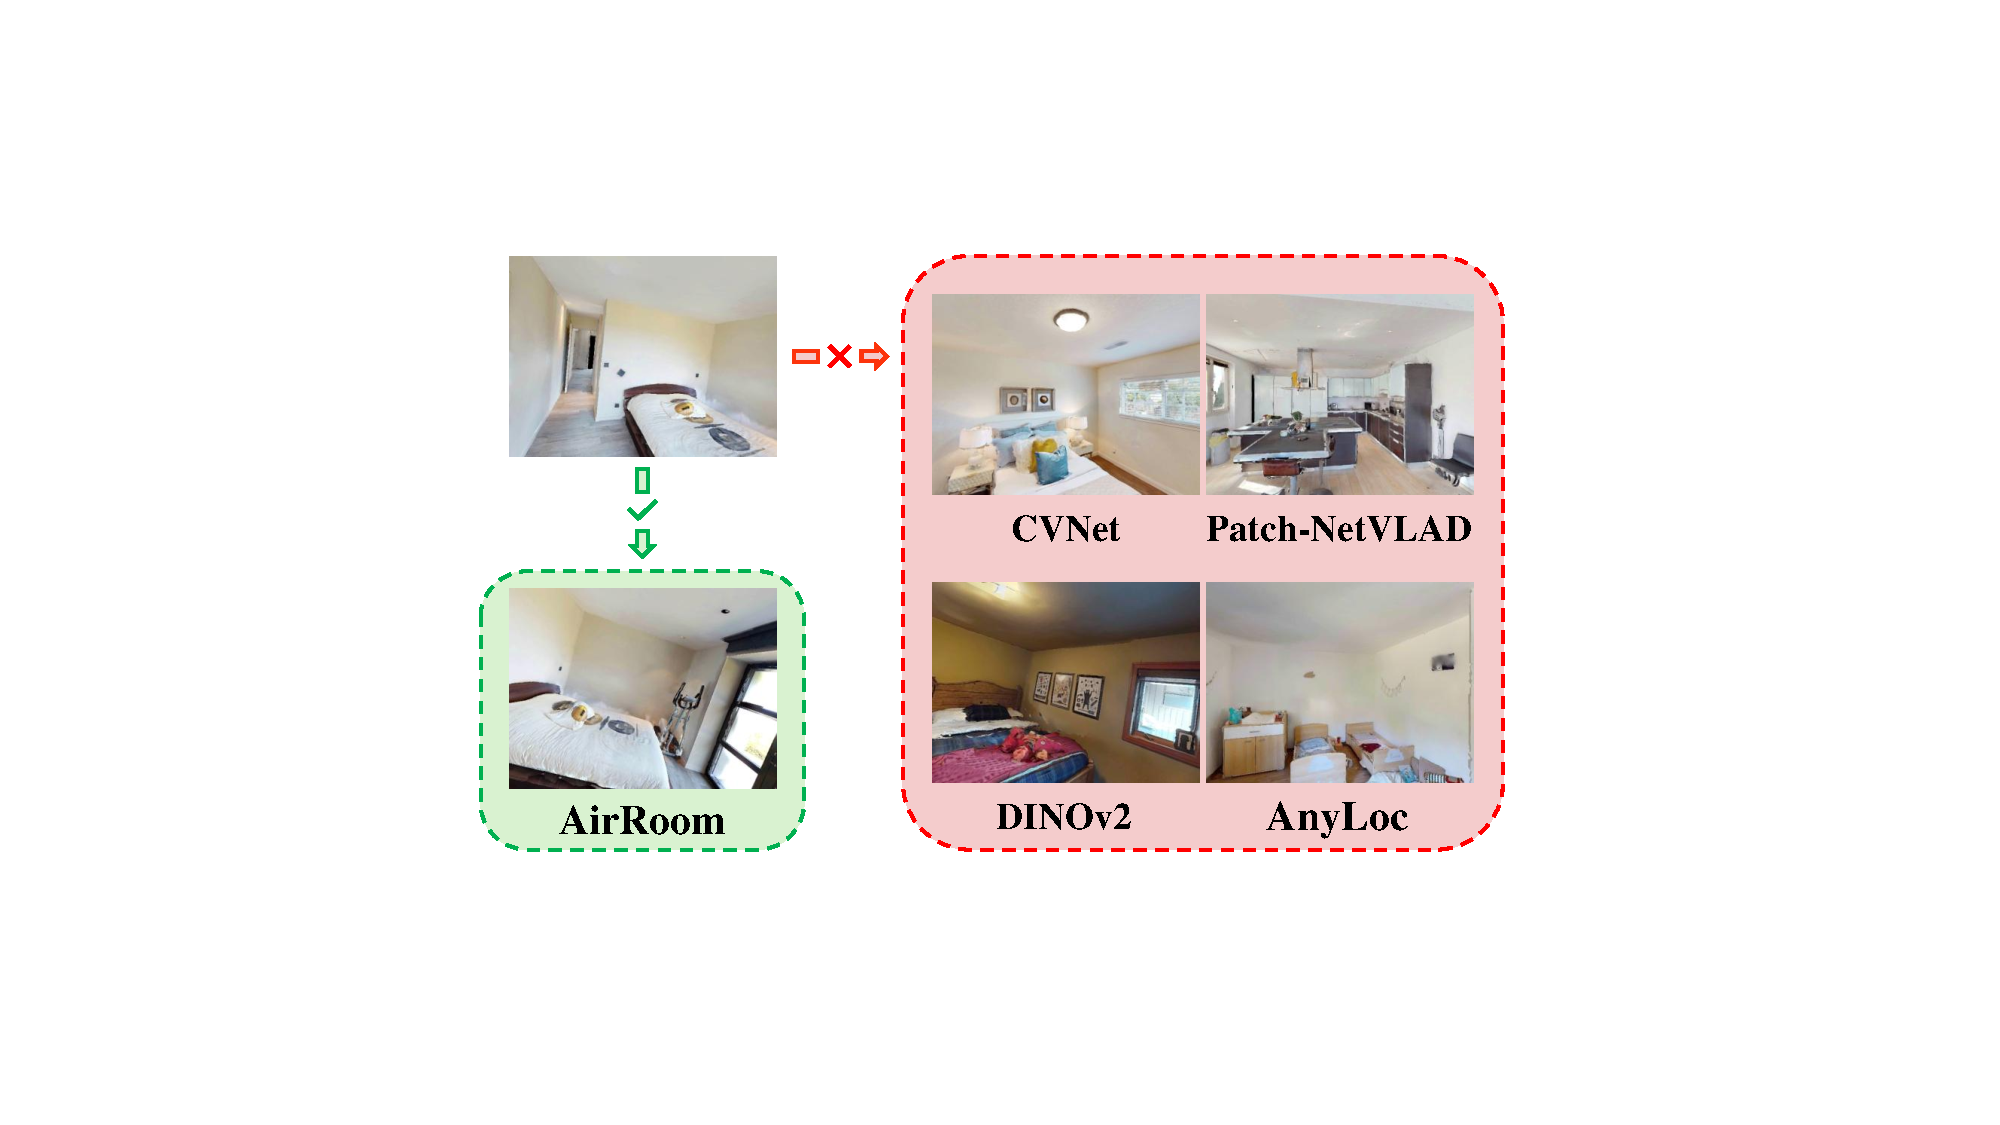
\includegraphics[width=\columnwidth]{failure_font.pdf}
    \vspace{-16pt}
    \caption{Given a bedroom query, AirRoom accurately retrieves the target image by leveraging object relevance for room reidentification. In contrast, CVNet retrieves visually similar images without preserving scene accuracy, DINOv2 captures semantic content but overlooks color details, Patch-NetVLAD, using aggregated local features to form global descriptors, retrieves images with mismatched semantic information, and AnyLoc considers semantic and color attributes but neglects object importance within rooms.}
    \vspace{-5pt}
    \label{fig:failure}
\end{figure}

\tref{tab:overall} presents a quantitative comparison between AirRoom and baseline methods, showing that AirRoom outperforms all baselines on nearly all metrics and datasets. In room reidentification tasks, image retrieval methods generally exhibit lower classification metrics due to their focus not being on top-1 precision, while VPR methods yield better results. Global descriptor-based VPR methods capture only high-level semantic information, often retrieving rooms with similar semantics but lacking detailed features. In contrast, VPR methods using aggregated local features, such as Patch-NetVLAD, emphasize low-level encodings but may overlook global context, resulting in less accurate retrievals. \fref{fig:failure} illustrates failure cases for CVNet, DINOv2, Patch-NetVLAD, and AnyLoc, highlighting these limitations. 
Although AnyLoc, known for its robust performance in ``anywhere, anytime, anyview" VPR, performs well, AirRoom further enhances performance, achieving a 20\% to 40\% improvement within the available margin compared to AnyLoc. For instance, AnyLoc achieves 89.69\% accuracy on HMReID, leaving approximately 10\% room for improvement. AirRoom, with an accuracy of 93.80\%, demonstrates up to a 40\% improvement within this remaining margin. These results highlight AirRoom's superior precision and refinement in room reidentification.

% \vspace{-4pt}
\subsection{Group-Wise Performance Comparison}
\label{sec:section4.5}
\vspace{-3pt}
Many baseline methods adopt a “backbone + enhancement mechanism” paradigm, which our approach also follows. In this section, we compare the performance of our object-aware enhancement mechanism with that of several state-of-the-art methods, using the same backbone as each group’s baseline. This setup allows us to directly assess the effectiveness of our object-aware enhancement mechanism.

For the ResNet50 backbone group, we use CVNet \cite{lee2022correlationverificationimageretrieval} as the baseline. In the NetVLAD backbone group, we employ Patch-NetVLAD \cite{hausler2021patchnetvladmultiscalefusionlocallyglobal} as the baseline, testing it at three reduction dimensions: 4096, 512, and 128.

\tref{tab:grouped} reveals that within each group, the single backbone outperforms the baseline methods that attempt to enhance performance through various mechanisms, indicating that these mechanisms do not effectively capture critical information in indoor rooms. In contrast, our object-aware enhancement mechanism significantly improves the backbone’s performance by emphasizing the importance of \mbox{objects} in indoor environments.

% \vspace{-4pt}
\subsection{Pipeline Flexibility Evaluation}
\label{sec:section4.6}
\vspace{-3pt}
In this section, we systematically evaluate the flexibility and adaptability of AirRoom by testing different configurations of its key modules. The results clearly demonstrate that AirRoom is not reliant on any specific model and can effectively integrate a diverse range of models.

\vspace{-5pt}
\subsubsection{Global Feature Extractor}
\vspace{-4pt}
We test various Global Feature Extractors, including ViT \cite{dosovitskiy2021imageworth16x16words}, DINO \cite{caron2021emergingpropertiesselfsupervisedvision}, DINOv2 \cite{oquab2024dinov2learningrobustvisual}, and AnyLoc-VLAD-DINOv2 \cite{keetha2023anylocuniversalvisualplace} with VLAD cluster sizes of 16 and 8.

As shown in \tref{tab:global feature extractor flexibility}, AirRoom consistently achieves over 85\% across all metrics and datasets in nearly every case, regardless of the capabilities of the Global Feature Extractor used. Even in the single exception with DINOv2, AirRoom still improves performance by nearly 15\%. This demonstrates that the effectiveness of our pipeline is not reliant on any specific Global Feature Extractor, highlighting AirRoom's adaptability to various backbone configurations and underscoring its robust flexibility.


\vspace{-5pt}
\subsubsection{Instance Segmentation}
\vspace{-4pt}
We compare traditional instance segmentation methods, such as Mask R-CNN \cite{he2018maskrcnn}, with more recent approaches, including Semantic-SAM \cite{li2023semanticsamsegmentrecognizegranularity}, which leverage advanced techniques for more granular segmentation.

\tref{tab:is flexibility} shows that AirRoom consistently outperforms the baseline by over 15\%, regardless of the instance segmentation module used. This demonstrates that our pipeline is not dependent on any specific instance segmentation method, underscoring its adaptability in this component.

\begin{table}[h]
\vspace{-5pt}
\centering
\resizebox{\columnwidth}{!}{%
\begin{tabular}{l|cccc}
\toprule
\multirow{2}{*}{\textbf{Methods}} & \multicolumn{4}{c}{\textbf{HMReID}} \\
 & Accuracy & Precision & Recall & F1 \\
\midrule
DINOv2 & 53.91 & 60.52 & 53.73 & 54.69 \\
\rowcolor{Lavender} AirRoom-MaskRCNN & 69.44 & 72.23 & 69.08 & 69.07 \\
\rowcolor{Lavender} AirRoom-SSAM & \textbf{70.95} & \textbf{73.86} & \textbf{70.66} & \textbf{70.78} \\
\bottomrule
\end{tabular}%
}
\vspace{-10pt}
\caption{Instance Segmentation Flexibility.}
\vspace{-16pt}
\label{tab:is flexibility}
\end{table}



\subsubsection{Object Feature Extractor}

We experiment with both traditional backbones, such as ResNet50 \cite{he2015deepresiduallearningimage}, and more modern backbones, like DINOv2 \cite{oquab2024dinov2learningrobustvisual}, as the Object Feature Extractor.

As shown in \tref{tab:ofe flexibility}, AirRoom achieves substantial performance improvements over the baseline, with minimal performance variation between different Object Feature Extractors. This supports the flexibility of our pipeline in accommodating a range of feature extraction methods.

\begin{table}[h]
\vspace{-6pt}
\centering
\resizebox{\columnwidth}{!}{%
\begin{tabular}{l|cccc}
\toprule
\multirow{2}{*}{\textbf{Methods}} & \multicolumn{4}{c}{\textbf{HMReID}} \\
 & Accuracy & Precision & Recall & F1 \\
\midrule
DINOv2 & 53.91 & 60.52 & 53.73 & 54.69 \\
\rowcolor{Lavender} AirRoom-ResNet50 & \textbf{70.95} & \textbf{73.86} & \textbf{70.66} & \textbf{70.78} \\
\rowcolor{Lavender} AirRoom-DINOv2 & 68.67 & 71.81 & 68.33 & 68.59 \\
\bottomrule
\end{tabular}%
}
\vspace{-10pt}
\caption{Object Feature Extractor Flexibility.}
\vspace{-20pt}
\label{tab:ofe flexibility}
\end{table}





\subsubsection{Object-Aware Scoring}

We evaluate both the mean (\(s_{\text{mean}}\)) and max (\(s_{\max}\)) strategies for computing the patch score (\(s_{\text{patch}}\)) and object score (\(s_{\text{object}}\)), assessing their impact on the overall performance.

\tref{tab:os flexibility} shows that AirRoom’s performance remains stable regardless of the object-aware scoring method used. This underscores the robustness of object-oriented information in room reidentification and demonstrates AirRoom’s flexibility in adapting to different scoring strategies.

\begin{table}[h]
\vspace{-6pt}
\centering
\resizebox{\columnwidth}{!}{%
\begin{tabular}{l|cccc}
\toprule
\multirow{2}{*}{\textbf{Methods}} & \multicolumn{4}{c}{\textbf{HMReID}} \\
 & Accuracy & Precision & Recall & F1 \\
\midrule
DINOv2 & 53.91 & 60.52 & 53.73 & 54.69 \\
\rowcolor{Lavender} AirRoom-Max(patch)-Mean(object) & 70.95 & 73.86 & 70.66 & 70.78 \\
\rowcolor{Lavender} AirRoom-Max(patch)-Max(object) & \textbf{71.02} & \textbf{74.02} & \textbf{70.72} & \textbf{70.85} \\
\rowcolor{Lavender} AirRoom-Mean(patch)-Max(object) & 70.85 & 73.85 & 70.55 & 70.70 \\
\rowcolor{Lavender} AirRoom-Mean(patch)-Mean(object) & 70.90 & 73.78 & 70.62 & 70.73 \\
\bottomrule
\end{tabular}%
}
\vspace{-10pt}
\caption{Object-Aware Scoring Flexibility.}
\vspace{-20pt}
\label{tab:os flexibility}
\end{table}


\subsection{Ablation Studies}
\label{sec:section4.7}

In this section, we remove certain modules from our pipeline—including the global score \(s_{\text{global}}\),  the patch score \(s_{\text{patch}}\), the object score \(s_{\text{object}}\), within object-aware scoring, and the entire Fine-Grained Retrieval (FGR)—to assess the importance and effectiveness of each component.

\begin{table}[t]
\centering
\resizebox{\columnwidth}{!}{%
\begin{tabular}{l|cccc}
\toprule
\multirow{2}{*}{\textbf{Methods}} & \multicolumn{4}{c}{\textbf{HMReID}} \\
 & Accuracy & Precision & Recall & F1 \\
\midrule
DINOv2 (AirRoom-w/o all)& 53.91 & 60.52 & 53.73 & 54.69 \\
\rowcolor{Lavender} AirRoom-w/o \(s_{\text{patch}}\) & 66.68 & 70.04 & 66.42 & 66.68 \\
\rowcolor{Lavender} AirRoom-w/o \(s_{\text{object}}\) & 69.77 & 72.84 & 69.48 & 69.64 \\
\rowcolor{Lavender} AirRoom-w/o FGR & 66.11 & 70.85 & 65.80 & 66.41 \\
\rowcolor{Lavender} AirRoom-w/o \(s_{\text{patch}}\) \& \(s_{\text{object}}\) & 62.26 & 66.43 & 62.03 & 62.46 \\
\rowcolor{Lavender} AirRoom-w/o \(s_{\text{patch}}\) \& FGR & 59.39 & 65.25 & 59.14 & 59.97 \\
\rowcolor{Lavender} AirRoom-w/o \(s_{\text{object}}\) \& FGR & 63.44 & 68.68 & 63.14 & 63.84 \\
\rowcolor{Lavender} AirRoom & \textbf{70.95} & \textbf{73.86} & \textbf{70.66} & \textbf{70.78} \\
\bottomrule
\end{tabular}%
}
\vspace{-10pt}
\caption{Ablation Studies (Excluding Global Score Experiments).}
\vspace{-6pt}
\label{tab:ablation w/o global score}
\end{table}

\begin{table}[ht]
\centering
\resizebox{\columnwidth}{!}{%
\begin{tabular}{l|cccc}
\toprule
\multirow{2}{*}{\textbf{Methods}} & \multicolumn{4}{c}{\textbf{HMReID}} \\
 & Accuracy & Precision & Recall & F1 \\
\midrule
ViT & 76.47 & 79.37 & 76.04 & 75.91 \\
\rowcolor{Lavender} AirRoom-ViT-w/o \(s_{\text{global}}\) & 84.86 & 86.82 & 84.34 & 84.61 \\
\rowcolor{Lavender} AirRoom-ViT & \textbf{86.58} & \textbf{88.13} & \textbf{86.12} & \textbf{86.23} \\
\cdashline{1-5}
DINOv2 & 53.91 & 60.52 & 53.73 & 54.69 \\
\rowcolor{Lavender} AirRoom-DINOv2-w/o \(s_{\text{global}}\) & \textbf{71.73} & \textbf{74.97} & \textbf{71.44} & \textbf{71.64} \\
\rowcolor{Lavender} AirRoom-DINOv2 & 70.95 & 73.86 & 70.66 & 70.78 \\
\bottomrule
\end{tabular}%
}
\vspace{-10pt}
\caption{Ablation Studies on Global Score.}
\vspace{-15pt}
\label{tab:ablation on global score}
\end{table}

\tref{tab:ablation w/o global score} shows that removing any module from our pipeline leads to a performance drop. However, as long as at least one module remains, our pipeline still outperforms the baseline. \tref{tab:ablation on global score}  demonstrates that when the Global Feature Extractor (ViT) performs well, the global score \(s_{\text{global}}\) significantly enhances performance. On the other hand, when the Global Feature Extractor (DINOv2) is less effective, the global score \(s_{\text{global}}\) has a slight negative impact, causing a small drop in performance. This result aligns with our hypothesis in Section~\ref{subsec:refinement}, where the global score acts as a prior to rank the priority of the five candidates. Overall, these ablation studies confirm that every module in our pipeline is both important and necessary.

\subsection{Limitations}

While AirRoom achieves state-of-the-art performance in room reidentification under various viewpoint variations, a limitation of our work is the inability to verify robustness to indoor object rearrangements caused by movable objects. Although our mutual nearest neighbors-based Object-Aware Scoring method is somewhat robust to such rearrangements, the datasets used in our experiments lack these cases. In contrast, recent advances in dynamic scene understanding \cite{zhao2024dynamicsceneunderstandingobjectcentric} focus on recognizing scenes in the presence of moving objects, potentially offering greater robustness than our approach. Future work should consider constructing datasets that include object rearrangements and integrating new techniques to enhance robustness to movable objects, thereby improving room reidentification.
\vspace{-5pt}
\section{Conclusion}
\vspace{-5pt}
\label{sec:conclusion}

Room reidentification is a challenging yet crucial research area, with growing applications in fields like augmented reality and homecare robotics. In this paper, we introduce AirRoom, a training-free, object-aware approach for room reidentification. AirRoom leverages multi-level object-oriented features to capture both spatial and contextual information of indoor rooms. To evaluate AirRoom, we constructed four novel datasets specifically for room reidentification. Experimental results demonstrate its robustness to viewpoint variations and superior performance over state-of-the-art methods across nearly all metrics and datasets. Furthermore, the pipeline is highly flexible, maintaining high performance without relying on specific model configurations. Collectively, our work establishes AirRoom as a powerful and versatile solution for precise room reidentification, with broad potential for real-world applications.

\begin{center}
\textbf{Acknowledgments}  
\end{center}
% This work was partially supported by the DARPA grant DARPA-PS-23-13. The views and conclusions contained in this document are those of the authors and should not be interpreted as representing the official policies, either expressed or implied, of DARPA.
\begin{sloppypar}
\noindent This work was supported by the DARPA award HR00112490426. Any opinions, findings, conclusions, or recommendations expressed in this paper are those of the authors and do not necessarily reflect the views of DARPA.
\end{sloppypar}


% \input{sec/8_formatting}
% \input{sec/9_finalcopy}
{
    \small
    \bibliographystyle{ieeenat_fullname}
    \bibliography{main}
}

% WARNING: do not forget to delete the supplementary pages from your submission 
\clearpage
\appendix
\setcounter{page}{1}
\maketitlesupplementary

\section{Implementation Details}
We follow prior studies\cite{coop, cocoop, prograd, kgcoop, maple, tcp, mma} and adopt a 16-shot learning setting across all experiments, except for the few-shot learning tasks. The ViT-B/16\cite{vit} variant of the CLIP model serves as the visual backbone for all experimental setups. Hand-crafted text prompts from prior methods\cite{clip, coop, tip-adapter} are utilized and described in detail in \cref{datasets}. Optimization is performed using the AdamW optimizer with an initial learning rate of 0.001. All our models are trained with mix-precision for speeding up. For the larger ImageNet dataset, we employ a batch size of 32, while a batch size of 4 is used for all other datasets. Training on ImageNet for the base-to-novel generalization task spans 5 epochs, whereas training on the remaining datasets is conducted over 10 epochs. For cross-dataset evaluation and domain generalization tasks, we perform training for a single epoch on ImageNet. In the few-shot learning tasks, training is carried out for 5 epochs on ImageNet and 50 epochs for other datasets. The average accuracy is reported over three independent runs, with all experiments executed on a single NVIDIA RTX 4090 GPU.

Representation tokens are initialized from a zero-mean Gaussian distribution with a standard deviation of 0.02. We set $J = 6$, integrating the representation tokens beginning at the 6-th transformer layer. The dimension of the representation space, $d_r$, is set to 2048 for EuroSAT and 512 for all other datasets. Note that since the $d_r$ setting for EuroSAT differs from other datasets, in the $d_r$ ablation experiments we fix $d_r$ for EuroSAT to 2048 while adjusting $d_r$ on the other datasets. The number of representation tokens, $K$, is configured to 5. The parameter $\alpha$ is fixed at 0.7, and the details regarding the configuration of $\lambda$ are provided in \cref{ablation_lambda}.



\section{Dataset Details}
Details of 14 datasets are shown in \cref{datasets}.


\section{Computational Cost}
Table \ref{computational_cost} summarizes the learnable parameters, training time per image, total training duration, inference speed (measured in frames per second, FPS, with a batch size of 100), and the final HM metric for each approach. Our proposed model, MMRL, demonstrates a compelling balance of computational efficiency and performance. The key observations are as follows:
\begin{itemize}
    \item Models incorporating multimodal interaction mechanisms (e.g., MaPLe, MMA, and MMRL) generally involve a higher parameter count compared to models without such mechanisms.
    \item Both MMRL and the prior MMA approach exhibit significantly faster training speed, thereby reducing overall computational costs. While MaPLe and PromptSRC achieve higher inference speeds, their training durations are relatively longer. Notably, MMRL offers faster inference compared to MMA and MetaPrompt.
    \item To assess the performance of MMRL under constrained computational resources, we reduced the dimensionality of the representation space from 512 to 32. In this configuration, MMRL achieves a parameter count comparable to that of MMA, while still significantly outperforming the previous state-of-the-art model.
\end{itemize}



\begin{table}[h]
\centering
\renewcommand\arraystretch{1.25}
\caption{All methods were trained on a single NVIDIA RTX 4090 GPU using the ImageNet dataset. Each model was implemented with publicly available code and default configurations as described in their respective papers \cite{maple, promptsrc, provp, metaprompt, tcp, mma}. `V-L' denotes vision-language interaction, indicating that efficient fine-tuning incorporates interactions between visual and textual modalities before prediction. `V, L' signifies separate fine-tuning of each modality without inter-modal interaction before prediction, while `L' refers to fine-tuning limited to the textual modality alone. `Train time' is reported as both time per image and the total duration for training the full dataset(16-shots), while `FPS (100 BS)' indicates frames per second with a batch size of 100 during inference.}
\label{computational_cost}
\resizebox{0.475\textwidth}{!}{
    \begin{tabular}{@{}l|ccccc|c@{}}
    \toprule
    \multirow{2}{*}{Method} & \multirow{2}{*}{Modality} & Params & Train time & Train time & FPS & \multirow{2}{*}{HM} \\
               &     & (learnable) & (ms/image) & (minute/all) & (100 BS) &       \\ \midrule
    MaPLe      & V-L & 3.555M      & 39.5       & 26.4         & 1757.6   & 78.55 \\
    PromptSRC  & V,L & 0.046M      & 40.0       & 106.8        & 1764.2   & 79.97 \\
    ProVP      & V   & 0.147M      & 4.4        & 107.2        & 928.9    & 78.76 \\
    MetaPrompt & V,L & 0.031M      & 30.7       & 32.8         & 659.8    & 79.09 \\
    TCP        & L   & 0.332M      & 5.3        & 17.7         & 950.6    & 79.51 \\
    MMA        & V-L & 0.675M      & 2.2        & 1.5          & 688.5    & 79.87 \\ \midrule
    MMRL       & V-L & 4.992M      & 5.3        & 3.6          & 762.4    & 81.20 \\
    MMRL*      & V-L & 0.689M      & 5.3        & 3.6          & 767.8    & 80.84 \\ \bottomrule
    \end{tabular}
}
\end{table}


\section{Ablation Analysis on $\lambda$}
As shown in \cref{ablation_lambda}, increasing the value of $\lambda$ generally improves performance, with the optimal or near-optimal results typically observed when $\lambda$ is set between 4 and 6 across most datasets. Notably, as $\lambda$ continues to increase, its impact on model performance within the same dataset diminishes, indicating reduced sensitivity to variations in $\lambda$. This trend suggests that the model becomes more robust and less reliant on precise tuning of $\lambda$ at higher values.


\begin{table*}[h]
\centering
\caption{Summary of the 14 datasets.}
\label{datasets}
\renewcommand\arraystretch{1.2}
\resizebox{1.0\textwidth}{!}{
    \begin{tabular}{@{}l|llllll@{}}
    \toprule
    Dataset      & Classes & Train  & Val    & Test   & Description                         & Prompt                                \\ \midrule
    ImageNet     & 1000    & 1.28M  & $\sim$ & 50000  & Recognition of generic objects      & ``a photo of a [CLASS].”              \\
    Caltech101   & 100     & 4128   & 1649   & 2465   & Recognition of generic objects      & ``a photo of a [CLASS].”              \\
    OxfordPets      & 37    & 2944   & 736    & 3669   & Fine-grained classification of pets                    & ``a photo of a [CLASS], a type of pet.”      \\
    StanfordCars & 196     & 6509   & 1635   & 8041   & Fine-grained classification of cars & ``a photo of a [CLASS].”              \\
    Flowers102      & 102   & 4093   & 1633   & 2463   & Fine-grained classification of flowers                 & ``a photo of a [CLASS], a type of flower.”   \\
    Food101         & 101   & 50500  & 20200  & 30300  & Fine-grained classification of foods                   & ``a photo of [CLASS], a type of food.”       \\
    FGVCAircraft    & 100   & 3334   & 3333   & 3333   & Fine-grained classification of aircrafts               & ``a photo of a [CLASS], a type of aircraft.” \\
    SUN397       & 397     & 15880  & 3970   & 19850  & Scene classification                & ``a photo of a [CLASS].”              \\
    DTD          & 47      & 2820   & 1128   & 1692   & Texture classification              & ``[CLASS] texture.”                   \\
    EuroSAT         & 10    & 13500  & 5400   & 8100   & Land use \& cover classification with satellite images & ``a centered satellite photo of [CLASS].”    \\
    UCF101       & 101     & 7639   & 1898   & 3783   & Action recognition                  & ``a photo of a person doing [CLASS].” \\ \midrule
    ImageNetV2   & 1,000   & $\sim$ & $\sim$ & 10,000 & New test data for ImageNet          & ``a photo of a [CLASS].”              \\
    ImageNet-Sketch & 1,000 & $\sim$ & $\sim$ & 50,889 & Sketch-style images of ImageNet classes                & ``a photo of a [CLASS].”                     \\
    ImageNet-A      & 200   & $\sim$ & $\sim$ & 7,500  & Natural adversarial examples of 200 ImageNet classes   & ``a photo of a [CLASS].”                     \\
    ImageNet-R   & 200     & $\sim$ & $\sim$ & 30,000 & Renditions of 200 ImageNet classes  & ``a photo of a [CLASS].”              \\ \bottomrule
    \end{tabular}
    }
\end{table*}


\begin{table*}[h]
\centering
\caption{Ablation on $\lambda$ across 11 datasets, with results evaluated using the harmonic mean (HM) metric.}
\label{ablation_lambda}
\renewcommand\arraystretch{1.2}
\resizebox{1.0\textwidth}{!}{
    \begin{tabular}{@{}c|ccccccccccc@{}}
    \toprule
    $\alpha$ & ImageNet       & Caltech101     & OxfordPets & StanfordCars & Flowers102 & Food101 & FGVCAircraft   & SUN397         & DTD            & EuroSAT & UCF101 \\ \midrule
    0.0  & 74.01 & 95.97 & 96.35          & 76.00          & 84.42          & 90.10          & 38.52 & 79.67 & 68.21 & 82.65          & 81.63          \\
    0.01 & 74.07 & 96.12 & 96.39          & 75.95          & 84.82          & 90.23          & 37.87 & 79.85 & 67.73 & \textbf{87.21} & 82.11          \\
    0.1  & 74.23 & 96.25 & 96.49          & 76.32          & 84.81          & 90.53          & 38.66 & 80.23 & 69.79 & 83.21          & 82.91          \\
    0.2  & 74.38 & 96.40 & \textbf{96.74} & 76.67          & 85.31          & 90.61          & 39.27 & 80.25 & 70.58 & 82.68          & 82.70          \\
    0.5      & \textbf{74.45} & \textbf{96.68} & 96.54      & 77.09        & 85.74      & 90.86   & 40.37          & 80.61          & 72.67          & 82.87   & 83.05  \\
    3.0  & 74.09 & 96.59 & 96.51          & 77.72          & 86.65          & 90.98          & 40.48 & 81.10 & 73.54 & 77.95          & \textbf{83.89} \\
    4.0  & 74.04 & 96.62 & 96.55          & 77.73          & \textbf{86.78} & 90.98          & 40.66 & 81.14 & 73.75 & 77.27          & 83.45          \\
    5.0  & 73.93 & 96.62 & 96.60          & 77.86          & 86.42          & \textbf{91.03} & 40.42 & 81.07 & 73.69 & 78.05          & 83.84          \\
    6.0      & 73.83          & 96.61          & 96.66      & 78.05        & 86.48      & 91.00   & \textbf{41.15} & \textbf{81.20} & \textbf{73.82} & 75.23   & 83.68  \\
    7.0  & 73.78 & 96.62 & 96.58          & \textbf{78.06} & 86.53          & 90.95          & 40.88 & 81.10 & 73.65 & 75.85          & 83.55          \\
    10.0 & 73.68 & 96.64 & 96.56          & 77.86          & 86.46          & 91.00          & 41.01 & 80.93 & 73.68 & 77.61          & 83.38          \\ \bottomrule
    \end{tabular}
}
\end{table*}

\begin{table}[t]
\small
\centering
\caption{Ablation on different regularization strategies.}
\label{ablation_regularization}
\begin{tabular}{@{}c|ccc@{}}
\toprule
Regularization & Base           & Novel          & HM             \\ \midrule
\rowcolor[HTML]{EFEFEF} 
Cosine         & \textbf{85.68} & \textbf{77.16} & \textbf{81.20} \\
L1             & 85.46          & 76.03          & 80.47          \\
MSE             & 85.13          & 74.62          & 79.53          \\ \bottomrule
\end{tabular}
\end{table}

\section{Ablation Analysis on Regularization Strategies}
We investigate the impact of various regularization strategies aimed at maximizing the similarity between class token features and frozen CLIP features to retain pre-trained knowledge. The results, summarized in \cref{ablation_regularization}, indicate that cosine regularization achieves the best performance. In contrast, both L1 and MSE losses lead to performance degradation, with MSE causing a significant decline. This result can be attributed to the more relaxed and flexible constraints of cosine regularization, enabling the class token to preserve generalizability while effectively capturing task-specific knowledge.






\section{Few-Shot Learning}
\cref{few_shot1,few_shot2} provide detailed comparisons of MMRL and prior state-of-the-art methods on few-shot learning across 11 datasets. MMRL achieves the highest average performance across all shots. Note that the MMA results are reproduced from the open-source code, as the original paper does not report results for this experiment.







\begin{table*}[t]
\small
\centering
\caption{Comparison of MMRL with previous state-of-the-art methods on few-shot learning across 11 datasets.}
\label{few_shot1}
\setlength{\tabcolsep}{15pt}{
\resizebox{0.9\textwidth}{!}{
    \begin{tabular}{@{}ll|ccccc}
    \toprule
    \textbf{Dataset} &
      \textbf{Method} &
      \textbf{1 shot} &
      \textbf{2 shots} &
      \textbf{4 shots} &
      \textbf{8 shots} &
      \textbf{16 shots} \\ \midrule
     &
      Linear probe CLIP &
      45.83 &
      57.98 &
      68.01 &
      74.47 &
      78.79 \\
     &
      CoOp &
      67.56 &
      70.65 &
      74.02 &
      76.98 &
      79.89 \\
     &
      CoCoOp &
      66.79 &
      67.65 &
      71.21 &
      72.96 &
      74.90 \\
     &
      MaPLe &
      69.27 &
      72.58 &
      75.37 &
      78.89 &
      81.79 \\
     &
      PromptSRC &
      72.32 &
      75.29 &
      78.35 &
      80.69 &
      82.87 \\
     &
      MMA &
      69.28 &
      72.08 &
      76.38 &
      79.57 &
      82.76 \\
    \multirow{-7}{*}{Average} &
      \cellcolor[HTML]{E8E8E8}$\text{MMRL}_{\text{ (Ours)}}$ &
      \cellcolor[HTML]{E8E8E8}\textbf{72.67} &
      \cellcolor[HTML]{E8E8E8}\textbf{75.90} &
      \cellcolor[HTML]{E8E8E8}\textbf{79.20} &
      \cellcolor[HTML]{E8E8E8}\textbf{81.47} &
      \cellcolor[HTML]{E8E8E8}\textbf{84.34} \\ \midrule
     &
      Linear probe CLIP &
      32.13 &
      44.88 &
      54.85 &
      62.23 &
      67.31 \\
     &
      CoOp &
      66.33 &
      67.07 &
      68.73 &
      70.63 &
      71.87 \\
     &
      CoCoOp &
      69.43 &
      69.78 &
      70.39 &
      70.63 &
      70.83 \\
     &
      MaPLe &
      62.67 &
      65.10 &
      67.70 &
      70.30 &
      72.33 \\
     &
      PromptSRC &
      68.13 &
      69.77 &
      71.07 &
      \textbf{72.33} &
      73.17 \\
     &
      MMA &
      \textbf{69.17} &
      \textbf{70.37} &
      71.00 &
      71.77 &
      73.13 \\
    \multirow{-7}{*}{ImageNet} &
      \cellcolor[HTML]{E8E8E8}$\text{MMRL}_{\text{ (Ours)}}$ &
      \cellcolor[HTML]{E8E8E8}69.00 &
      \cellcolor[HTML]{E8E8E8}70.30 &
      \cellcolor[HTML]{E8E8E8}\textbf{71.40} &
      \cellcolor[HTML]{E8E8E8}\textbf{72.33} &
      \cellcolor[HTML]{E8E8E8}\textbf{73.40} \\ \midrule
     &
      Linear probe CLIP &
      79.88 &
      89.01 &
      92.05 &
      93.41 &
      95.43 \\
     &
      CoOp &
      92.60 &
      93.07 &
      94.40 &
      94.37 &
      95.57 \\
     &
      CoCoOp &
      93.83 &
      94.82 &
      94.98 &
      95.04 &
      95.16 \\
     &
      MaPLe &
      92.57 &
      93.97 &
      94.43 &
      95.20 &
      96.00 \\
     &
      PromptSRC &
      93.67 &
      94.53 &
      95.27 &
      95.67 &
      96.07 \\
     &
      MMA &
      92.90 &
      94.00 &
      94.33 &
      95.37 &
      96.33 \\
    \multirow{-7}{*}{Caltech101} &
      \cellcolor[HTML]{E8E8E8}$\text{MMRL}_{\text{ (Ours)}}$ &
      \cellcolor[HTML]{E8E8E8}\textbf{94.17} &
      \cellcolor[HTML]{E8E8E8}\textbf{94.83} &
      \cellcolor[HTML]{E8E8E8}\textbf{96.03} &
      \cellcolor[HTML]{E8E8E8}\textbf{96.27} &
      \cellcolor[HTML]{E8E8E8}\textbf{97.13} \\ \midrule
     &
      Linear probe CLIP &
      44.06 &
      58.37 &
      71.17 &
      78.36 &
      85.34 \\
     &
      CoOp &
      90.37 &
      89.80 &
      92.57 &
      91.27 &
      91.87 \\
     &
      CoCoOp &
      91.27 &
      \textbf{92.64} &
      92.81 &
      93.45 &
      93.34 \\
     &
      MaPLe &
      89.10 &
      90.87 &
      91.90 &
      92.57 &
      92.83 \\
     &
      PromptSRC &
      \textbf{92.00} &
      92.50 &
      \textbf{93.43} &
      \textbf{93.50} &
      93.67 \\
     &
      MMA &
      91.23 &
      91.97 &
      92.23 &
      92.77 &
      93.23 \\
    \multirow{-7}{*}{OxfordPets} &
      \cellcolor[HTML]{E8E8E8}$\text{MMRL}_{\text{ (Ours)}}$ &
      \cellcolor[HTML]{E8E8E8}90.87 &
      \cellcolor[HTML]{E8E8E8}91.57 &
      \cellcolor[HTML]{E8E8E8}92.57 &
      \cellcolor[HTML]{E8E8E8}93.03 &
      \cellcolor[HTML]{E8E8E8}\textbf{93.83} \\ \midrule
     &
      Linear probe CLIP &
      35.66 &
      50.28 &
      63.38 &
      73.67 &
      80.44 \\
     &
      CoOp &
      67.43 &
      70.50 &
      74.47 &
      79.30 &
      83.07 \\
     &
      CoCoOp &
      67.22 &
      68.37 &
      69.39 &
      70.44 &
      71.57 \\
     &
      MaPLe &
      66.60 &
      71.60 &
      75.30 &
      79.47 &
      83.57 \\
     &
      PromptSRC &
      \textbf{69.40} &
      \textbf{73.40} &
      77.13 &
      80.97 &
      83.83 \\
     &
      MMA &
      67.87 &
      71.77 &
      76.50 &
      81.40 &
      85.70 \\
    \multirow{-7}{*}{StanfordCars} &
      \cellcolor[HTML]{E8E8E8}$\text{MMRL}_{\text{ (Ours)}}$ &
      \cellcolor[HTML]{E8E8E8}68.70 &
      \cellcolor[HTML]{E8E8E8}72.93 &
      \cellcolor[HTML]{E8E8E8}\textbf{78.17} &
      \cellcolor[HTML]{E8E8E8}\textbf{82.57} &
      \cellcolor[HTML]{E8E8E8}\textbf{86.43} \\ \midrule
     &
      Linear probe CLIP &
      69.74 &
      85.07 &
      92.02 &
      96.10 &
      97.37 \\
     &
      CoOp &
      77.53 &
      87.33 &
      92.17 &
      94.97 &
      97.07 \\
     &
      CoCoOp &
      72.08 &
      75.79 &
      78.40 &
      84.30 &
      87.84 \\
     &
      MaPLe &
      83.30 &
      88.93 &
      92.67 &
      95.80 &
      97.00 \\
     &
      PromptSRC &
      85.93 &
      91.17 &
      93.87 &
      96.27 &
      97.60 \\
     &
      MMA &
      83.60 &
      90.30 &
      93.00 &
      95.97 &
      97.97 \\
    \multirow{-7}{*}{Flowers102} &
      \cellcolor[HTML]{E8E8E8}$\text{MMRL}_{\text{ (Ours)}}$ &
      \cellcolor[HTML]{E8E8E8}\textbf{85.97} &
      \cellcolor[HTML]{E8E8E8}\textbf{91.20} &
      \cellcolor[HTML]{E8E8E8}\textbf{94.60} &
      \cellcolor[HTML]{E8E8E8}\textbf{96.60} &
      \cellcolor[HTML]{E8E8E8}\textbf{98.40} \\ \bottomrule
    \end{tabular}
    }
    }
\end{table*}


\begin{table*}[t]
\small
\centering
\caption{Comparison of MMRL with previous state-of-the-art methods on few-shot learning across 11 datasets.}
\label{few_shot2}
\setlength{\tabcolsep}{15pt}{
\resizebox{0.9\textwidth}{!}{
    \begin{tabular}{@{}ll|ccccc}
    \toprule
    \textbf{Dataset} &
      \textbf{Method} &
      \textbf{1 shot} &
      \textbf{2 shots} &
      \textbf{4 shots} &
      \textbf{8 shots} &
      \textbf{16 shots} \\ \midrule
     &
      Linear probe CLIP &
      43.96 &
      61.51 &
      73.19 &
      79.79 &
      82.90 \\
     &
      CoOp &
      84.33 &
      84.40 &
      84.47 &
      82.67 &
      84.20 \\
     &
      CoCoOp &
      \textbf{85.65} &
      \textbf{86.22} &
      \textbf{86.88} &
      \textbf{86.97} &
      87.25 \\
     &
      MaPLe &
      80.50 &
      81.47 &
      81.77 &
      83.60 &
      85.33 \\
     &
      PromptSRC &
      84.87 &
      85.70 &
      86.17 &
      86.90 &
      \textbf{87.50} \\
     &
      MMA &
      83.03 &
      82.50 &
      82.13 &
      83.00 &
      84.57 \\
    \multirow{-7}{*}{Food101} &
      \cellcolor[HTML]{E8E8E8}$\text{MMRL}_{\text{ (Ours)}}$ &
      \cellcolor[HTML]{E8E8E8}84.87 &
      \cellcolor[HTML]{E8E8E8}85.53 &
      \cellcolor[HTML]{E8E8E8}85.77 &
      \cellcolor[HTML]{E8E8E8}86.33 &
      \cellcolor[HTML]{E8E8E8}87.03 \\ \midrule
     &
      Linear probe CLIP &
      19.61 &
      26.41 &
      32.33 &
      39.35 &
      45.36 \\
     &
      CoOp &
      21.37 &
      26.20 &
      30.83 &
      39.00 &
      43.40 \\
     &
      CoCoOp &
      12.68 &
      15.06 &
      24.79 &
      26.61 &
      31.21 \\
     &
      MaPLe &
      26.73 &
      30.90 &
      34.87 &
      42.00 &
      48.40 \\
     &
      PromptSRC &
      27.67 &
      31.70 &
      37.47 &
      43.27 &
      50.83 \\
     &
      MMA &
      \textbf{28.73} &
      31.90 &
      37.57 &
      44.83 &
      52.70 \\
    \multirow{-7}{*}{FGVCAircraft} &
      \cellcolor[HTML]{E8E8E8}$\text{MMRL}_{\text{ (Ours)}}$ &
      \cellcolor[HTML]{E8E8E8}28.53 &
      \cellcolor[HTML]{E8E8E8}\textbf{34.23} &
      \cellcolor[HTML]{E8E8E8}\textbf{40.47} &
      \cellcolor[HTML]{E8E8E8}\textbf{48.07} &
      \cellcolor[HTML]{E8E8E8}\textbf{57.60} \\ \midrule
     &
      Linear probe CLIP &
      41.58 &
      53.70 &
      63.00 &
      69.08 &
      73.28 \\
     &
      CoOp &
      66.77 &
      66.53 &
      69.97 &
      71.53 &
      74.67 \\
     &
      CoCoOp &
      68.33 &
      69.03 &
      70.21 &
      70.84 &
      72.15 \\
     &
      MaPLe &
      64.77 &
      67.10 &
      70.67 &
      73.23 &
      75.53 \\
     &
      PromptSRC &
      \textbf{69.67} &
      \textbf{71.60} &
      \textbf{74.00} &
      75.73 &
      77.23 \\
     &
      MMA &
      64.00 &
      67.17 &
      69.97 &
      72.30 &
      74.63 \\
    \multirow{-7}{*}{SUN397} &
      \cellcolor[HTML]{E8E8E8}$\text{MMRL}_{\text{ (Ours)}}$ &
      \cellcolor[HTML]{E8E8E8}68.90 &
      \cellcolor[HTML]{E8E8E8}71.53 &
      \cellcolor[HTML]{E8E8E8}73.93 &
      \cellcolor[HTML]{E8E8E8}\textbf{76.00} &
      \cellcolor[HTML]{E8E8E8}\textbf{77.70} \\ \midrule
     &
      Linear probe CLIP &
      34.59 &
      40.76 &
      55.71 &
      63.46 &
      69.96 \\
     &
      CoOp &
      50.23 &
      53.60 &
      58.70 &
      64.77 &
      69.87 \\
     &
      CoCoOp &
      48.54 &
      52.17 &
      55.04 &
      58.89 &
      63.04 \\
     &
      MaPLe &
      52.13 &
      55.50 &
      61.00 &
      66.50 &
      71.33 \\
     &
      PromptSRC &
      56.23 &
      59.97 &
      65.53 &
      69.87 &
      72.73 \\
     &
      MMA &
      52.27 &
      56.90 &
      63.93 &
      67.97 &
      73.47 \\
    \multirow{-7}{*}{DTD} &
      \cellcolor[HTML]{E8E8E8}$\text{MMRL}_{\text{ (Ours)}}$ &
      \cellcolor[HTML]{E8E8E8}\textbf{56.37} &
      \cellcolor[HTML]{E8E8E8}\textbf{61.37} &
      \cellcolor[HTML]{E8E8E8}\textbf{67.87} &
      \cellcolor[HTML]{E8E8E8}\textbf{71.60} &
      \cellcolor[HTML]{E8E8E8}\textbf{75.30} \\ \midrule
     &
      Linear probe CLIP &
      49.23 &
      61.98 &
      77.09 &
      84.43 &
      87.21 \\
     &
      CoOp &
      54.93 &
      65.17 &
      70.80 &
      78.07 &
      84.93 \\
     &
      CoCoOp &
      55.33 &
      46.74 &
      65.56 &
      68.21 &
      73.32 \\
     &
      MaPLe &
      71.80 &
      78.30 &
      84.50 &
      87.73 &
      92.33 \\
     &
      PromptSRC &
      73.13 &
      79.37 &
      86.30 &
      \textbf{88.80} &
      92.43 \\
     &
      MMA &
      55.07 &
      59.80 &
      79.40 &
      86.47 &
      92.37 \\
    \multirow{-7}{*}{EuroSAT} &
      \cellcolor[HTML]{E8E8E8}$\text{MMRL}_{\text{ (Ours)}}$ &
      \cellcolor[HTML]{E8E8E8}\textbf{76.00} &
      \cellcolor[HTML]{E8E8E8}\textbf{82.87} &
      \cellcolor[HTML]{E8E8E8}\textbf{87.67} &
      \cellcolor[HTML]{E8E8E8}88.73 &
      \cellcolor[HTML]{E8E8E8}\textbf{93.37} \\ \midrule
     &
      Linear probe CLIP &
      53.66 &
      65.78 &
      73.28 &
      79.34 &
      82.11 \\
     &
      CoOp &
      71.23 &
      73.43 &
      77.10 &
      80.20 &
      82.23 \\
     &
      CoCoOp &
      70.30 &
      73.51 &
      74.82 &
      77.14 &
      78.14 \\
     &
      MaPLe &
      71.83 &
      74.60 &
      78.47 &
      81.37 &
      85.03 \\
     &
      PromptSRC &
      74.80 &
      \textbf{78.50} &
      81.57 &
      84.30 &
      86.47 \\
     &
      MMA &
      74.17 &
      76.17 &
      80.10 &
      83.43 &
      86.30 \\
    \multirow{-7}{*}{UCF101} &
      \cellcolor[HTML]{E8E8E8}$\text{MMRL}_{\text{ (Ours)}}$ &
      \cellcolor[HTML]{E8E8E8}\textbf{75.97} &
      \cellcolor[HTML]{E8E8E8}\textbf{78.50} &
      \cellcolor[HTML]{E8E8E8}\textbf{82.67} &
      \cellcolor[HTML]{E8E8E8}\textbf{84.67} &
      \cellcolor[HTML]{E8E8E8}\textbf{87.60} \\ \bottomrule
    \end{tabular}
    }
    }
\end{table*}




\end{document}
